% Default font is 11pt, which is pretty big, especially for internal
% talks Default aspect ratio is 4:3. "32", i.e. 3:2, is a compromise
% between 4:3 and 16:9
%
% Compromising on 3:2 is reasonable when you're going to show the talk
% on a projector and you don't know what kind of projector or screen it
% will be.
%
% 16:9 is best if others will be viewing it on their own devices,
% fullscreen.
%
% 4:3 is best if others will be viewing it on their own devices in a
% meeting where they want to also see the participants list/participant
% video/chat window.
%
% 3:2 is a good compromise when people will be viewing it on their own
% devices, but you don't know if they'll want to use part of the screen
% for something else or not.
%
% So 3:2 is the best default overall as of 2021. This may well change in
% the future.
%
\documentclass[aspectratio=32,10pt]{beamer}

% These together produce the same font as usual, but with copyable underscores
\usepackage[T1]{fontenc}

\usepackage{xspace}
\usepackage[absolute, overlay]{textpos}
\usepackage{verbatim}
\usepackage{graphicx}
\usepackage{array}

% Sets default width for includegraphics images
\setkeys{Gin}{width=\columnwidth}

\frenchspacing

\hypersetup{colorlinks}

\newcommand{\ul}{\begin{itemize}}
\newcommand{\lu}{\end{itemize}}
\newcommand{\ol}{\begin{enumerate}}
\newcommand{\lo}{\end{enumerate}}

\newcommand{\cols}{\begin{columns}}
\newcommand{\sloc}{\end{column}\end{columns}}

\newcommand{\col}{\begin{column}{0.5\textwidth}}
\newcommand{\colw}[1]{\begin{column}{#1\textwidth}}

\newcommand{\colbr}{\end{column}\begin{column}{0.5\textwidth}}
\newcommand{\colbrw}[1]{\end{column}\begin{column}{#1\textwidth}}

\newcommand{\hl}{$t_{1/2}$\xspace}

\newcommand{\is}[2]{\texorpdfstring{${}^{#1}$#2}{#2-#1}}

\newcommand{\meas}[4]{$(#1#2\mathrm{(stat)}#3\mathrm{(syst)})#4$}

\newcommand{\cn}{$^{\mathrm{[citation~needed]}}$\xspace}

\newcommand{\dedx}{$\mathrm{d}E/\mathrm{d}x$\xspace}
\newcommand{\piz}{$\pi^0$\xspace}
\newcommand{\pip}{$\pi^+$\xspace}
\newcommand{\pim}{$\pi^-$\xspace}
\newcommand{\mup}{$\mu^+$\xspace}
\newcommand{\mum}{\texorpdfstring{$\mu^-$\xspace}{mu\xspace}}

% "bold all" -- make both normal and math mode bold
\newcommand{\ba}[1]{{\boldmath \bf #1}}


\setbeamertemplate{navigation symbols}{} 
\mode<presentation>

% With minimal space usage for sections:
% default
% Boadilla
% Madrid
% Pittsburgh
% Rochester
%
% With space used at top for sections:
% AnnArbor
% Antibes
% Berlin
% CambridgeUS
% Copenhagen
% Darmstadt
% Dresden
% Frankfurt
% Ilmenau
% JuanLesPins
% Luebeck
% Montpellier
% Singapore
% Szeged
% Warsaw
%
% With space used on right or left for sections:
% Berkeley
% Goettingen
% Hannover
% Malmoe
% Marburg
% PaloAlto
%
% With space used on left for ... something:
% Bergen
\usetheme{PaloAlto}
% default
% albatross
% beaver
% beetle
% crane
% dolphin
% dove
% fly
% lily
% orchid
% rose
% seagull
% seahorse
% whale
% wolverine
\usecolortheme{default}

\setbeamersize{text margin left=2mm,text margin right=2mm} 

\author{Matthew Strait}
\institute{University of Minnesota}

%%%%%%%%%%
% Tricks %
%%%%%%%%%%

\newcommand{\beginbackup}{
   \newcounter{framenumbervorappendix}
   \setcounter{framenumbervorappendix}{\value{framenumber}}
}
\newcommand{\backupend}{
   \addtocounter{framenumbervorappendix}{-\value{framenumber}}
   \addtocounter{framenumber}{\value{framenumbervorappendix}} 
}

\newcommand{\topbit}[3]{
  \title[#3]{#1}
  \pdfinfo{
     /Author (Matthew Strait)
     /Title  (#1)
  }
  \date{#2}

  \begin{document}

  \frame{
   \maketitle
  }

}

\usepackage{tikz}

\newcommand{\hcancel}[1]{%
    \tikz[baseline=(tocancel.base)]{
        \node[inner sep=0pt,outer sep=0pt] (tocancel) {#1};
        \draw[black] (tocancel.west) -- (tocancel.east);
    }%
}%

\setbeamertemplate{footline}[frame number]


\topbit{LIGO follow-up progress}{29 Aug 2017}
       {GW, LIGO}

\section{Intro}

\frame{\frametitle{Outline}

\ul

\item Writing the code for our LIGO follow-up

\item Implements plan from \href{https://nova-docdb.fnal.gov/cgi-bin/private/ShowDocument?docid=22025}{doc-22025}

\item Testing on a randomly chosen timestamp

\item When satisfied, will turn it loose on the four LIGO events

\lu

}

\section{Middle}

\frame{\frametitle{Examine these triggers}

\ul

\item Near detector
  
  \ul

    \item BNB: Sometimes $\sim$0.27\% livetime for low energy events

    \item Activity: 100\% live for high energy events (what's the threshold?)

  \lu

\item Far detector

  \ul

    \item Periodic calibration pulser, a.k.a. 10\,Hz: 0.549\% live for low energy events

    \item Energy, contained vertex, Up-$\mu$, $\nu_\mu$: 100\% live for air showers, GeV neutrinos

    \item Fast, slow monopole: Don't expect monopoles, but could pick up something missed
          by the above

  \lu

\item Other triggers ignored for negligible livetime and/or non-useful acceptance

\item Would use DDsupernova if available, of course!

\lu

}

\frame{\frametitle{Rationale}

\ul

\item This is largely an exercise to prepare for future events

\item Tiny livetimes mean no chance of seeing a low-energy burst, especially 
since Super-K, Borexino and KamLAND have already reported null results

  \ul

  \item In the future, we can trigger on LIGO/VIRGO events and get 100\% livetime

  \lu

\item For triggered events, not as hopeless, but only
within phase space not excluded by Super-K

\lu

}

\frame{\frametitle{Testing}

\ul

\item Picked \mbox{2017-03-26 17:46:40.5 UTC} at random for testing

\item Most random pulser data is not reconstructed

\item I'm running just CalHit, Slicer4D, and BreakPointFitter (and its dependencies)

  \ul

    \item O(10s) per FD trigger, but only a few files

    \item Not clear how to get the full reco chain without preselection

    \item Also not clear that it's needed

  \lu

\item Simple set of histograms:

\ul

  \item Raw count of hits in each second of data

  \item Hits in the noise slice only

  \item Count of tracks

  \item Tracks with one end contained (mostly stoppers)

  \item Contained tracks

\lu

\lu

}

\frame{\frametitle{Far Detector pulser data}

\begin{center}

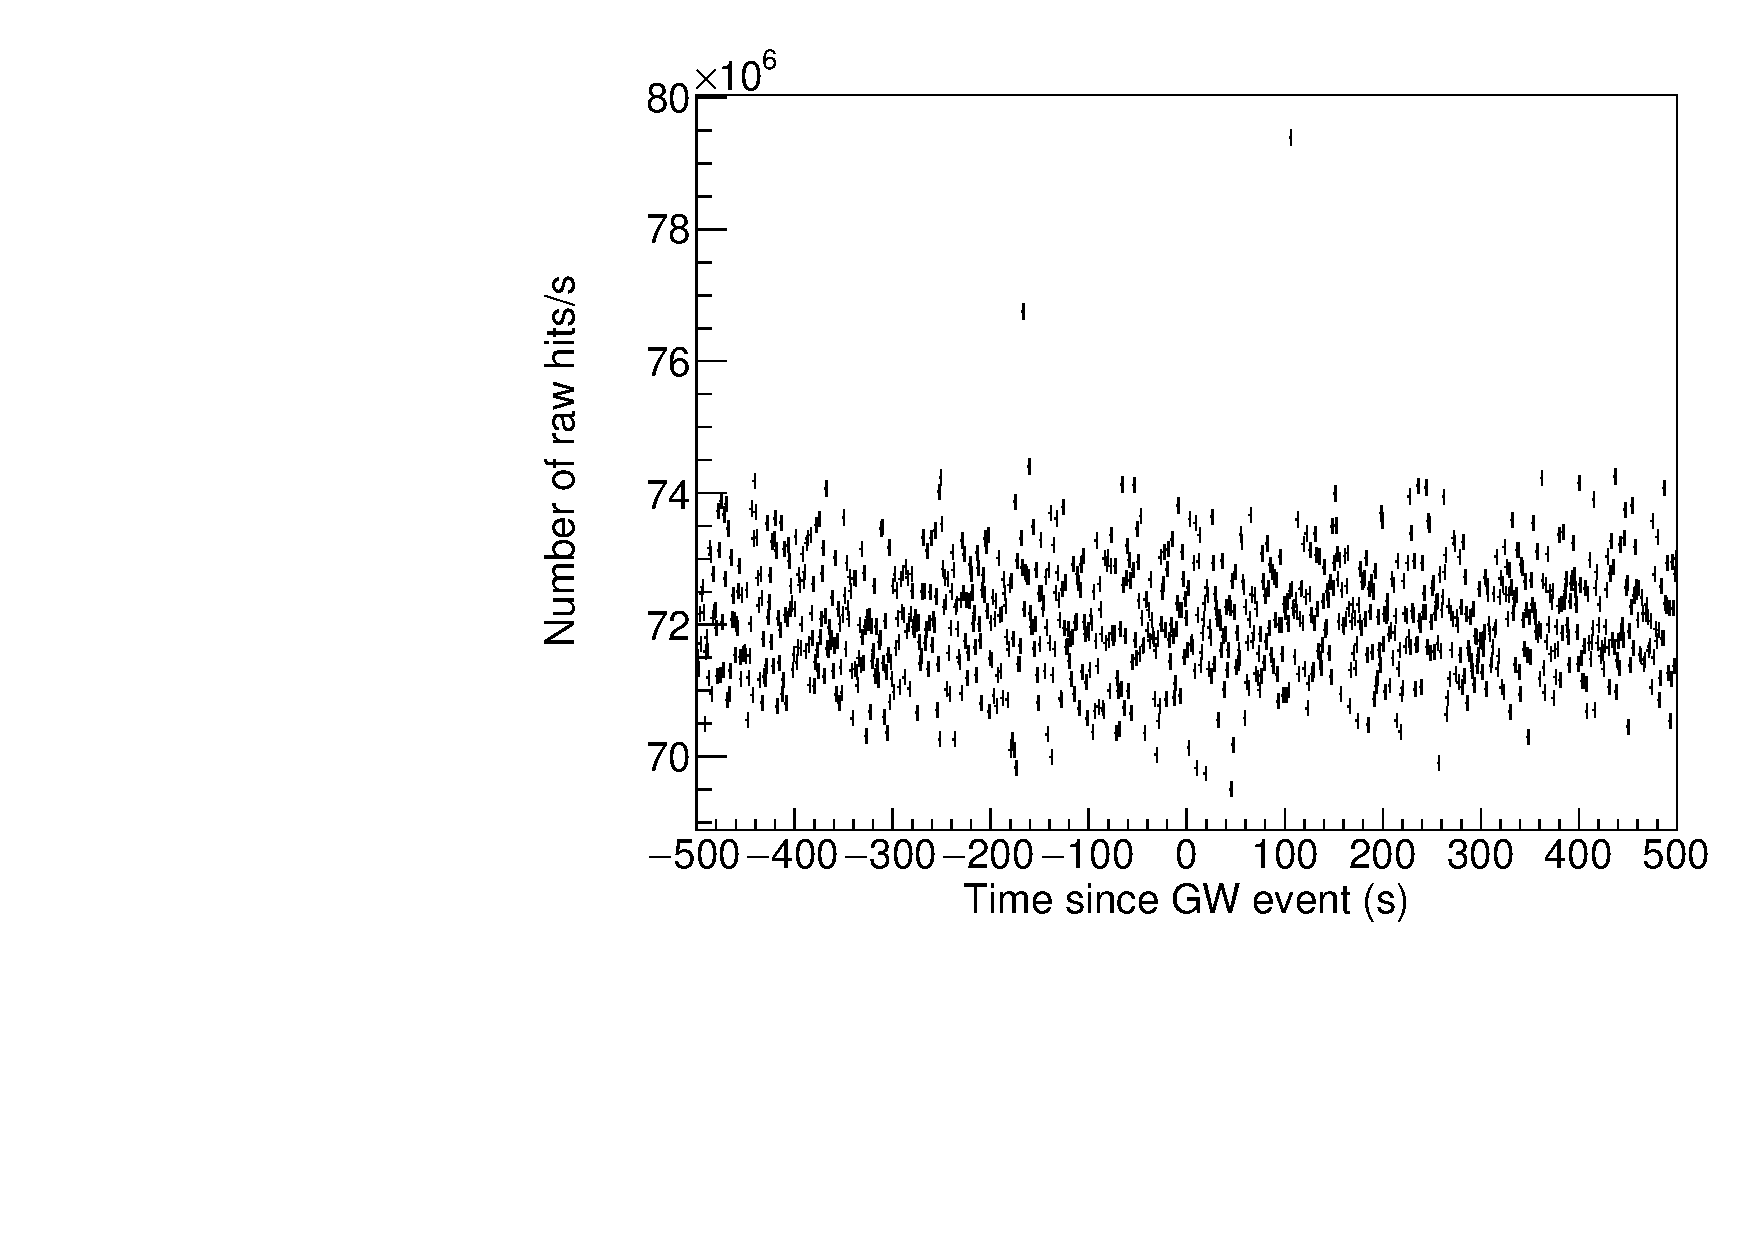
\includegraphics[width=0.333\columnwidth]{ligopass2-fardet-pulser-rawhits.pdf}%
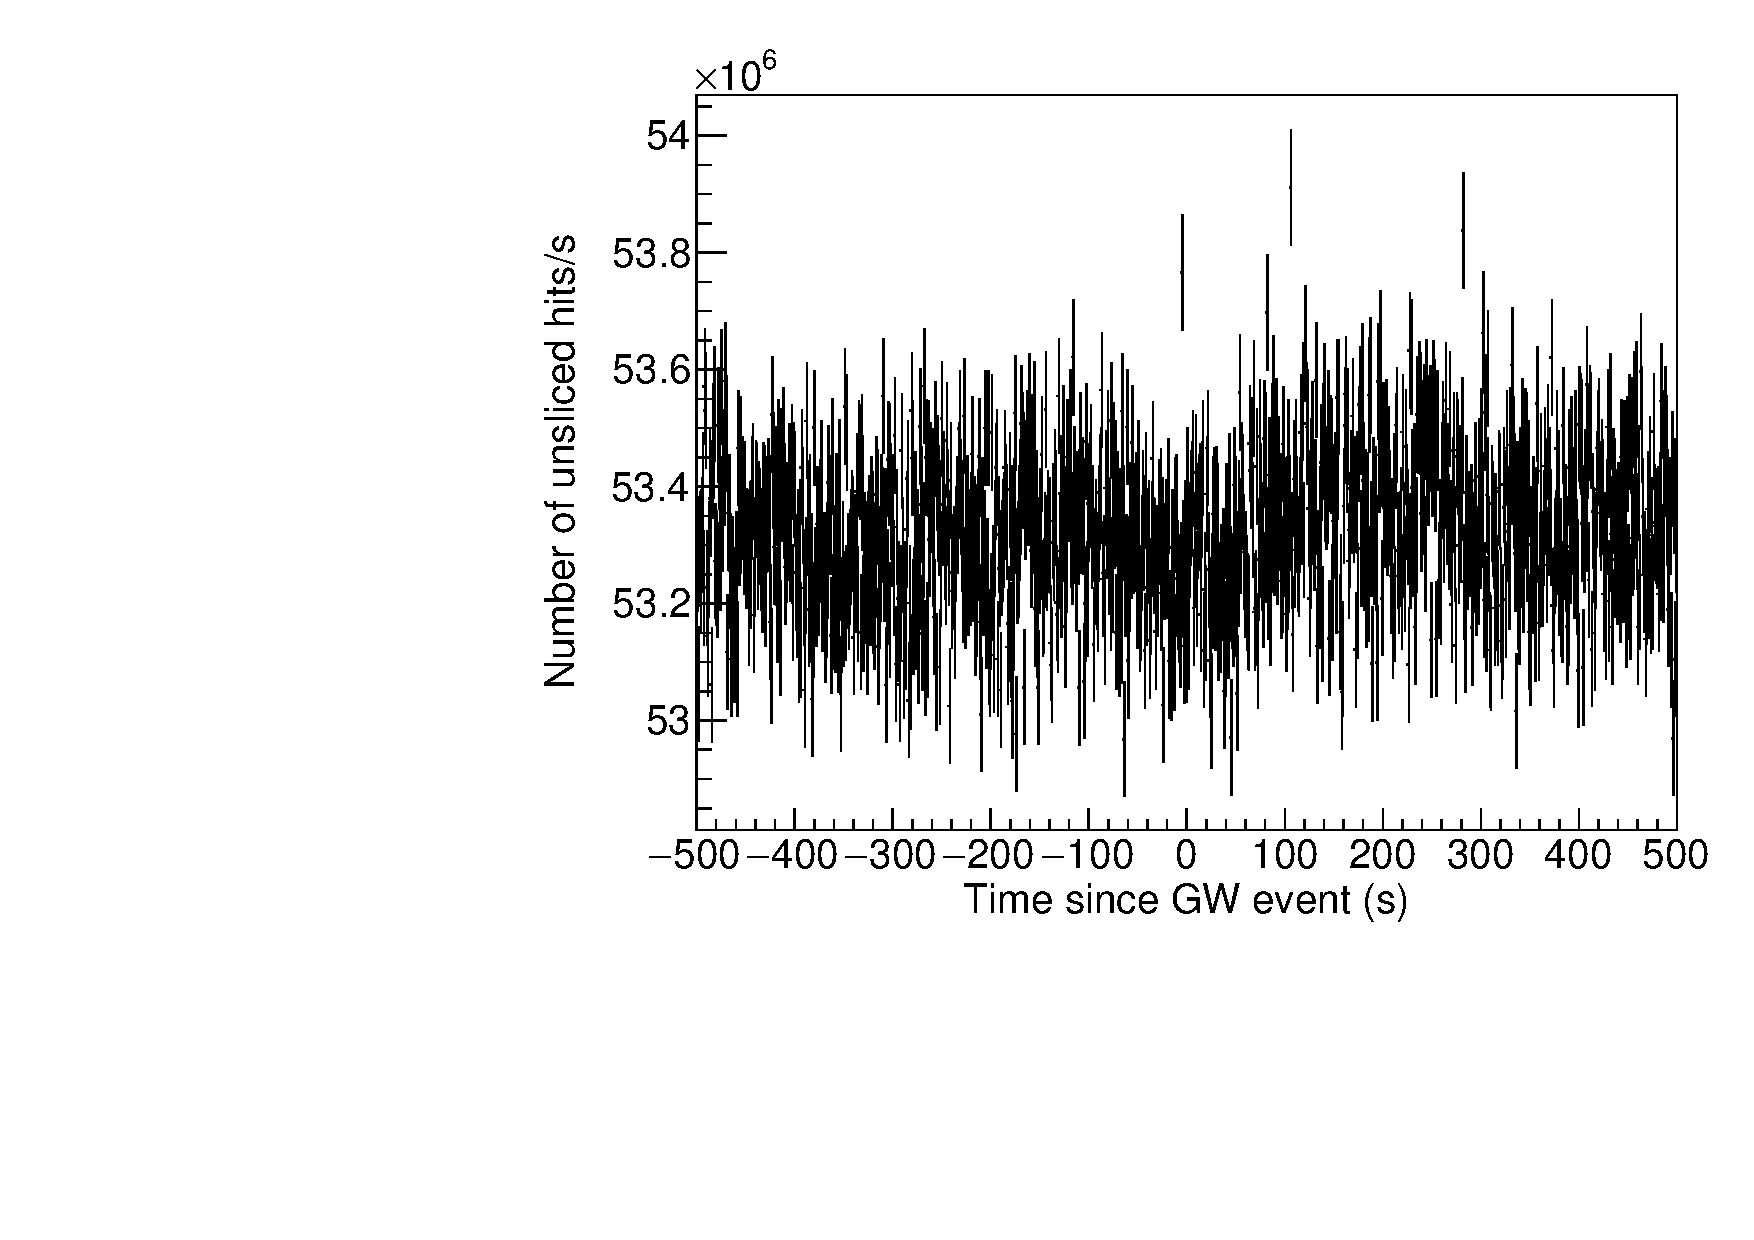
\includegraphics[width=0.333\columnwidth]{ligopass2-fardet-pulser-unslicedhits.pdf}

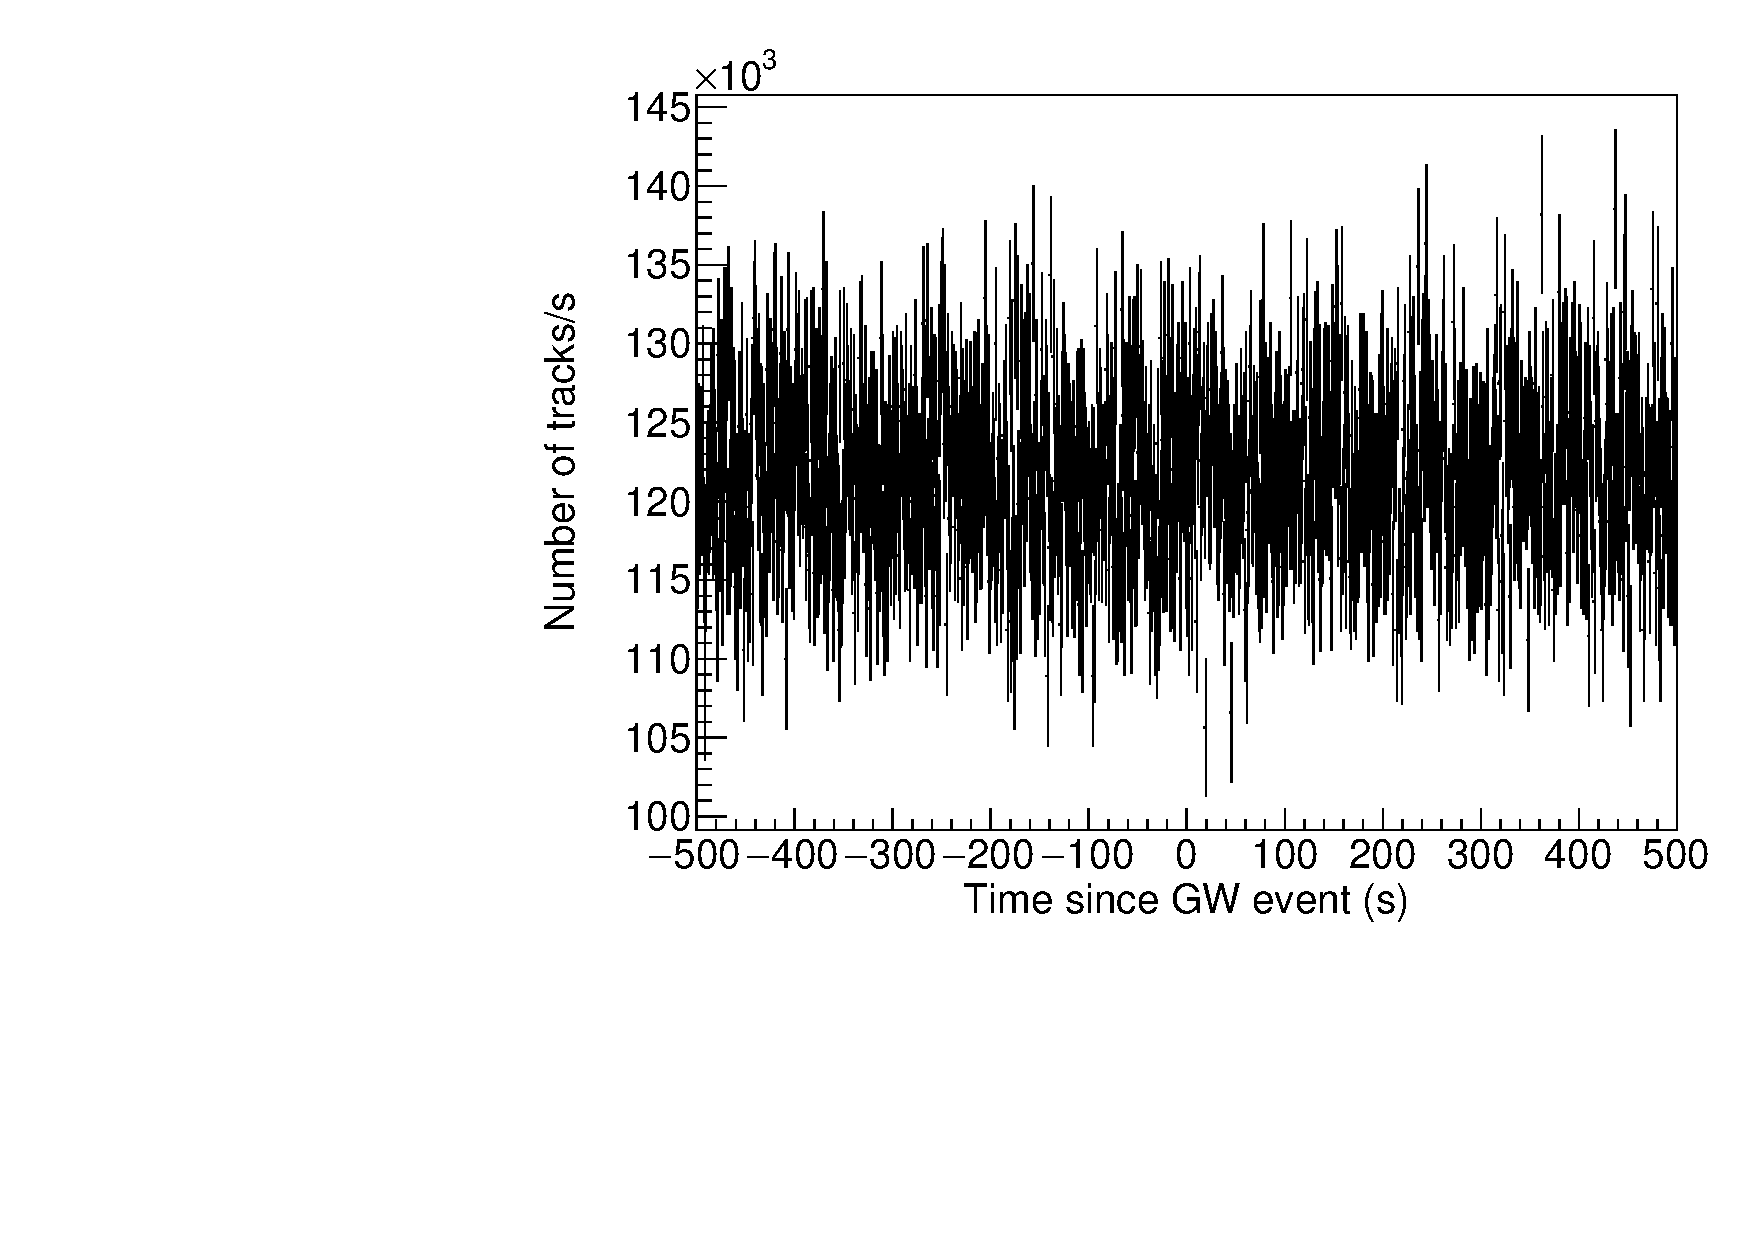
\includegraphics[width=0.333\columnwidth]{ligopass2-fardet-pulser-tracks.pdf}%
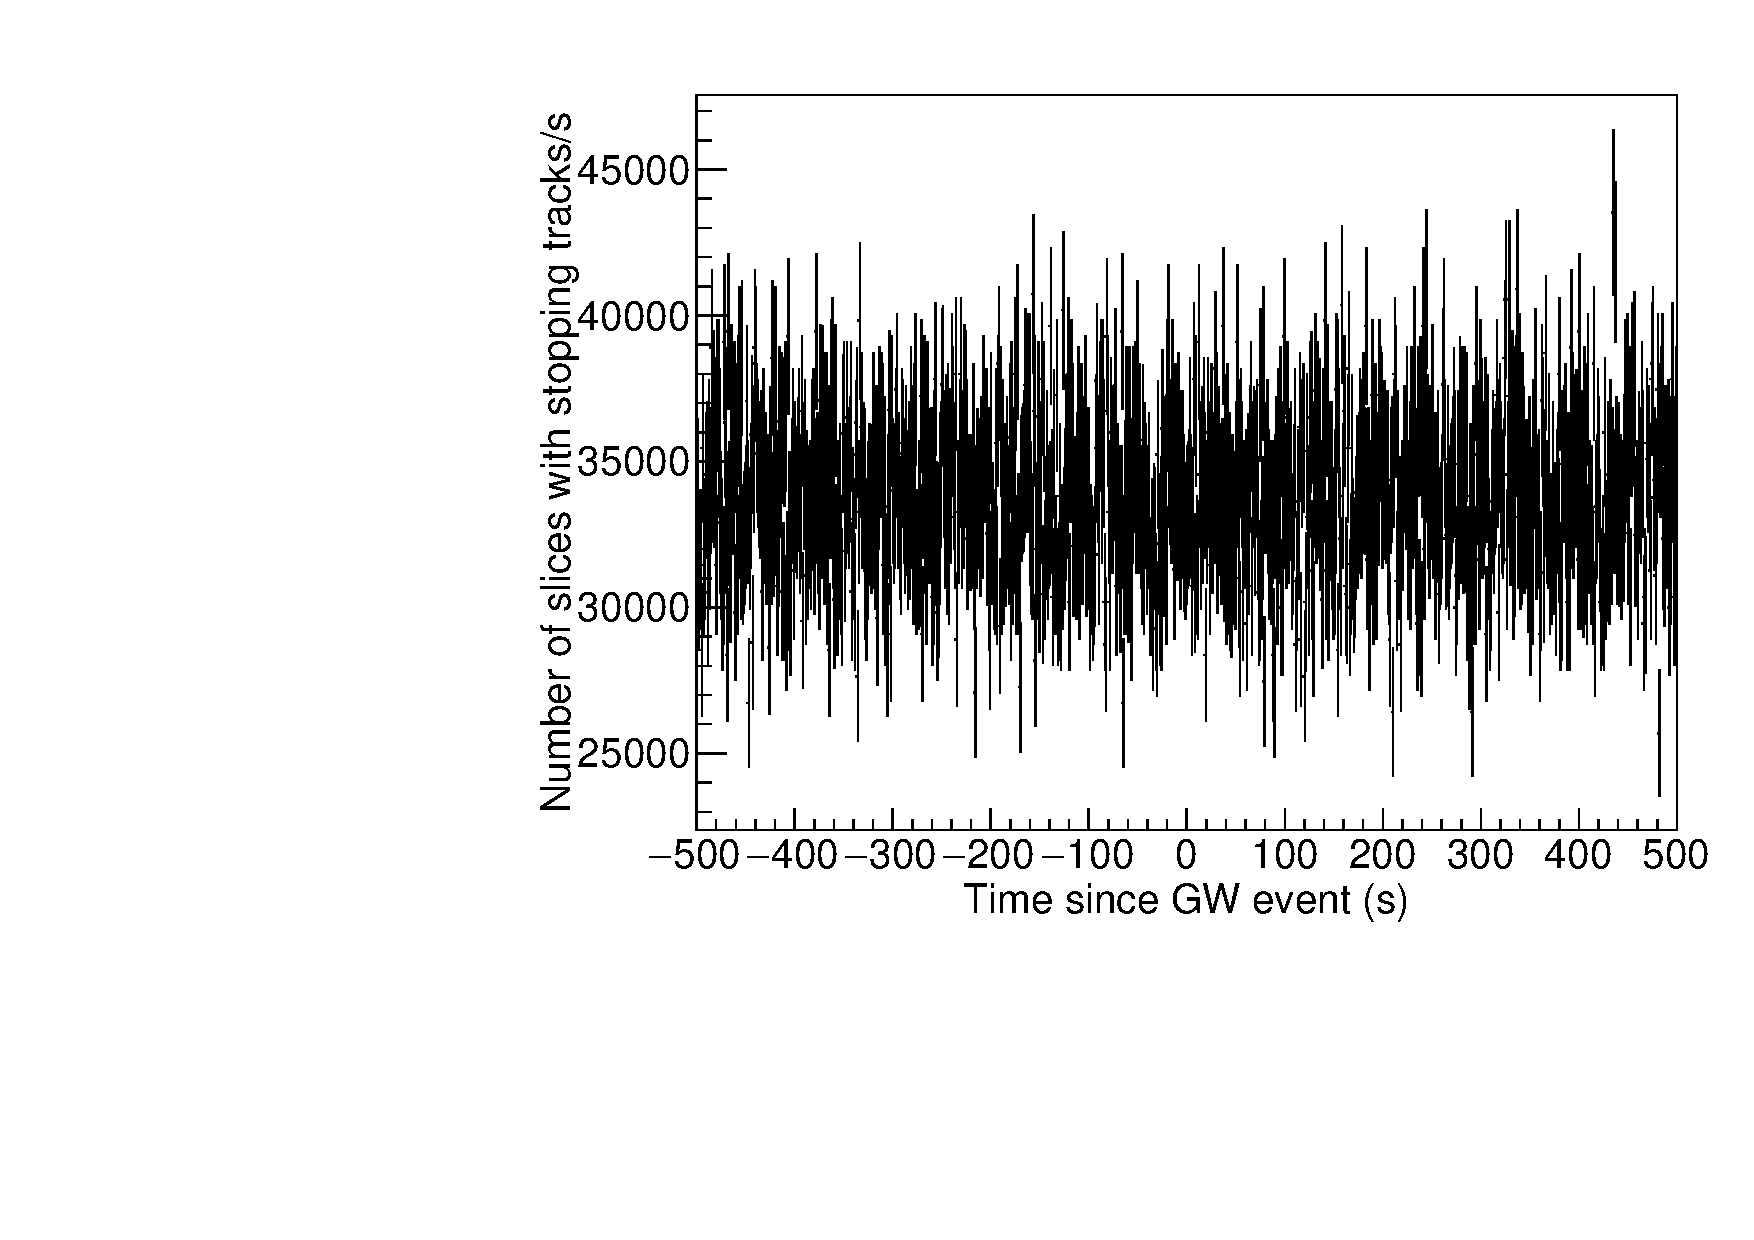
\includegraphics[width=0.333\columnwidth]{ligopass2-fardet-pulser-stoppingtracks.pdf}%
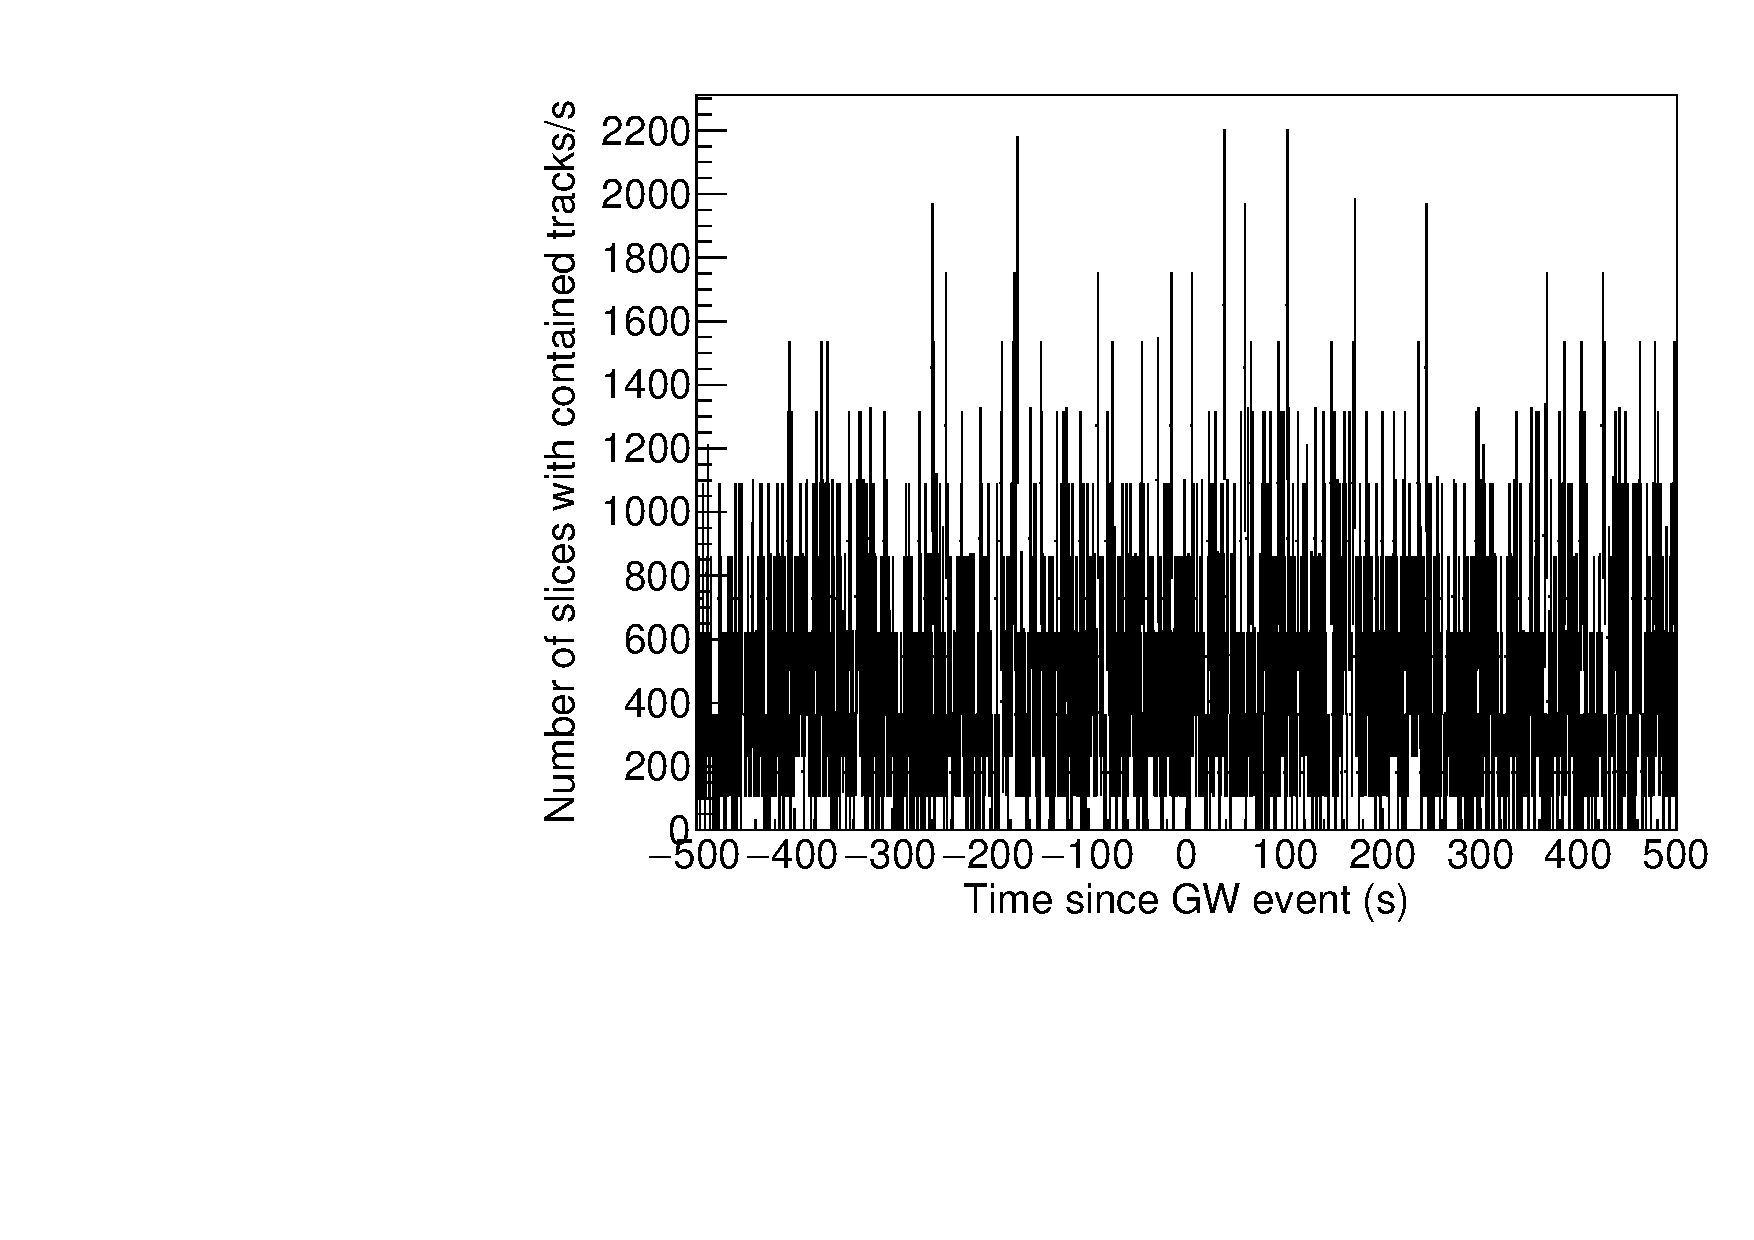
\includegraphics[width=0.333\columnwidth]{ligopass2-fardet-pulser-containedtracks.pdf}%

\end{center}

\ul

  \item .\phantom{tp}

\lu

}

\frame{\frametitle{Near Detector BNB}

\begin{center}

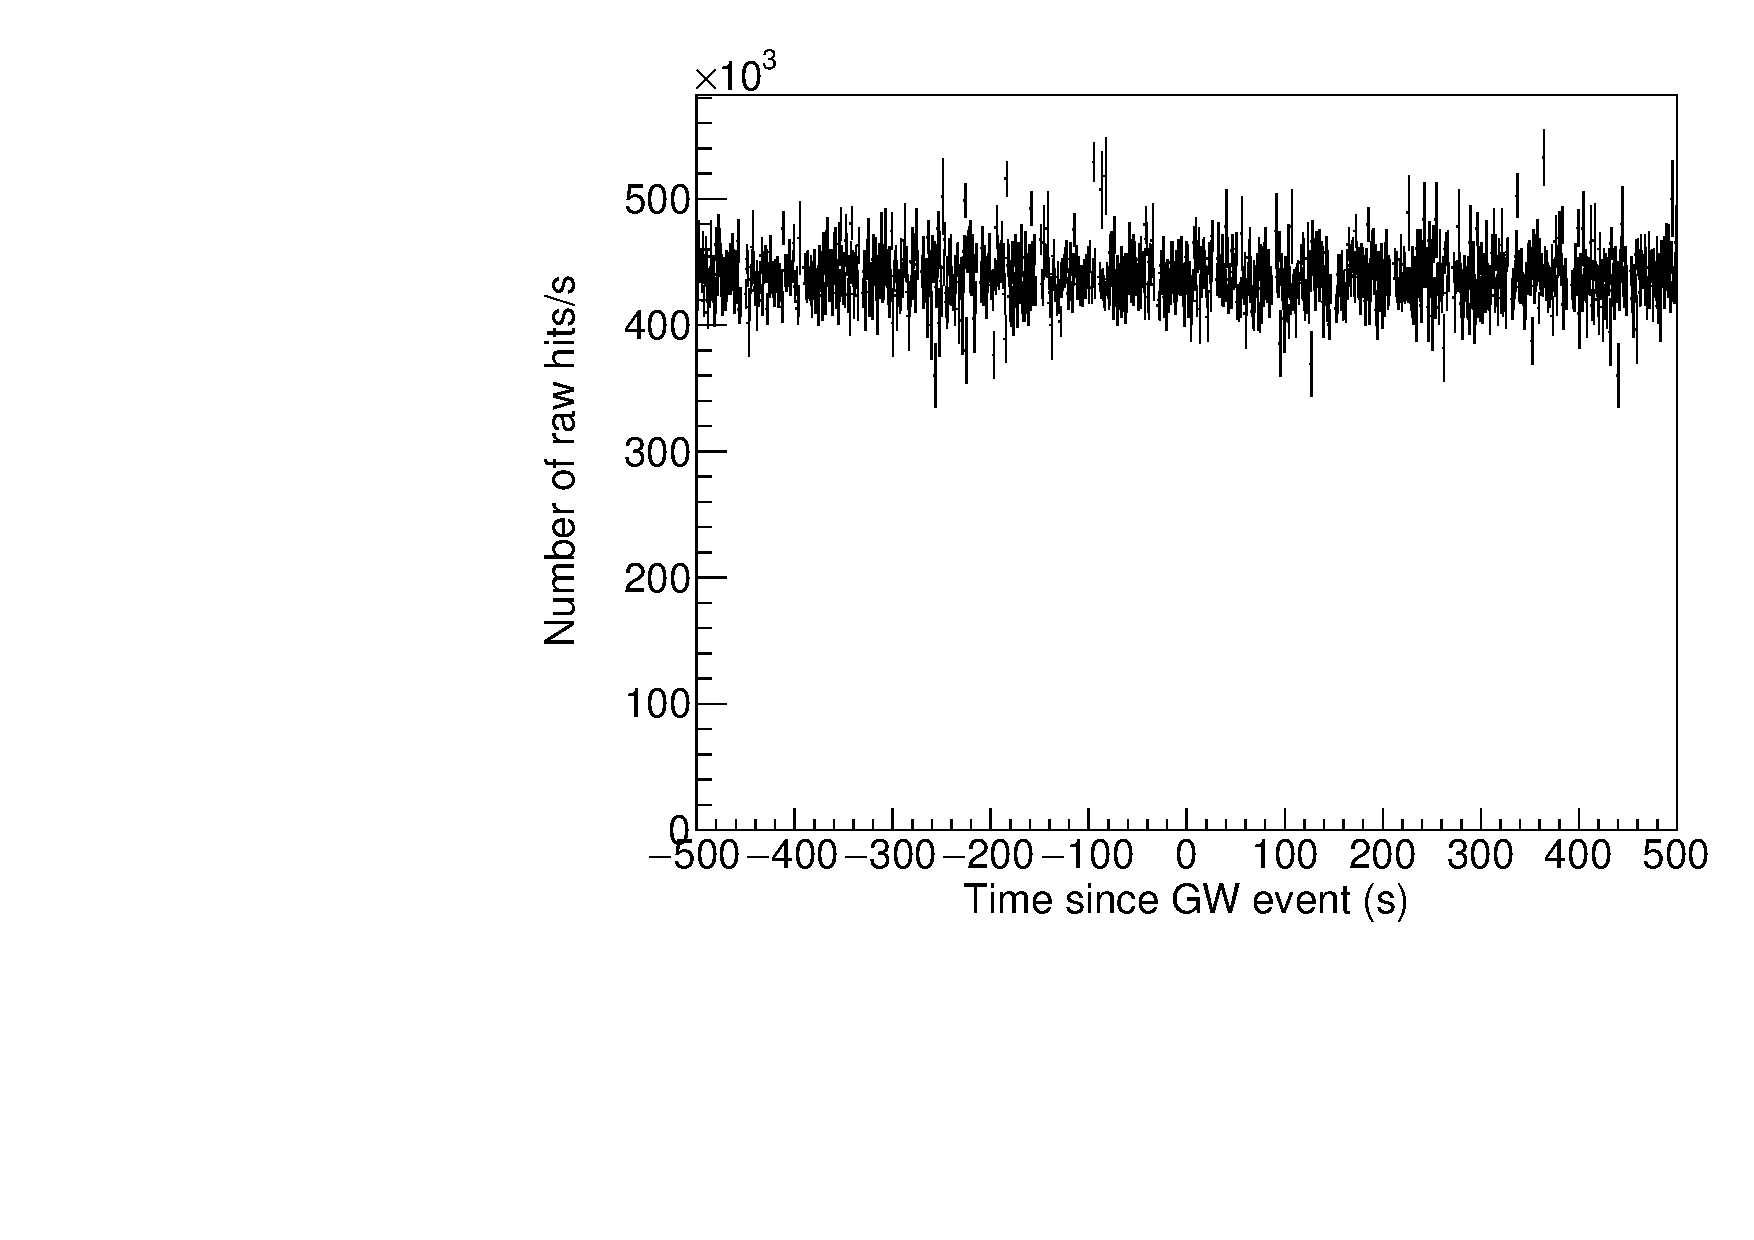
\includegraphics[width=0.333\columnwidth]{ligopass2-neardet-bnb-rawhits.pdf}%
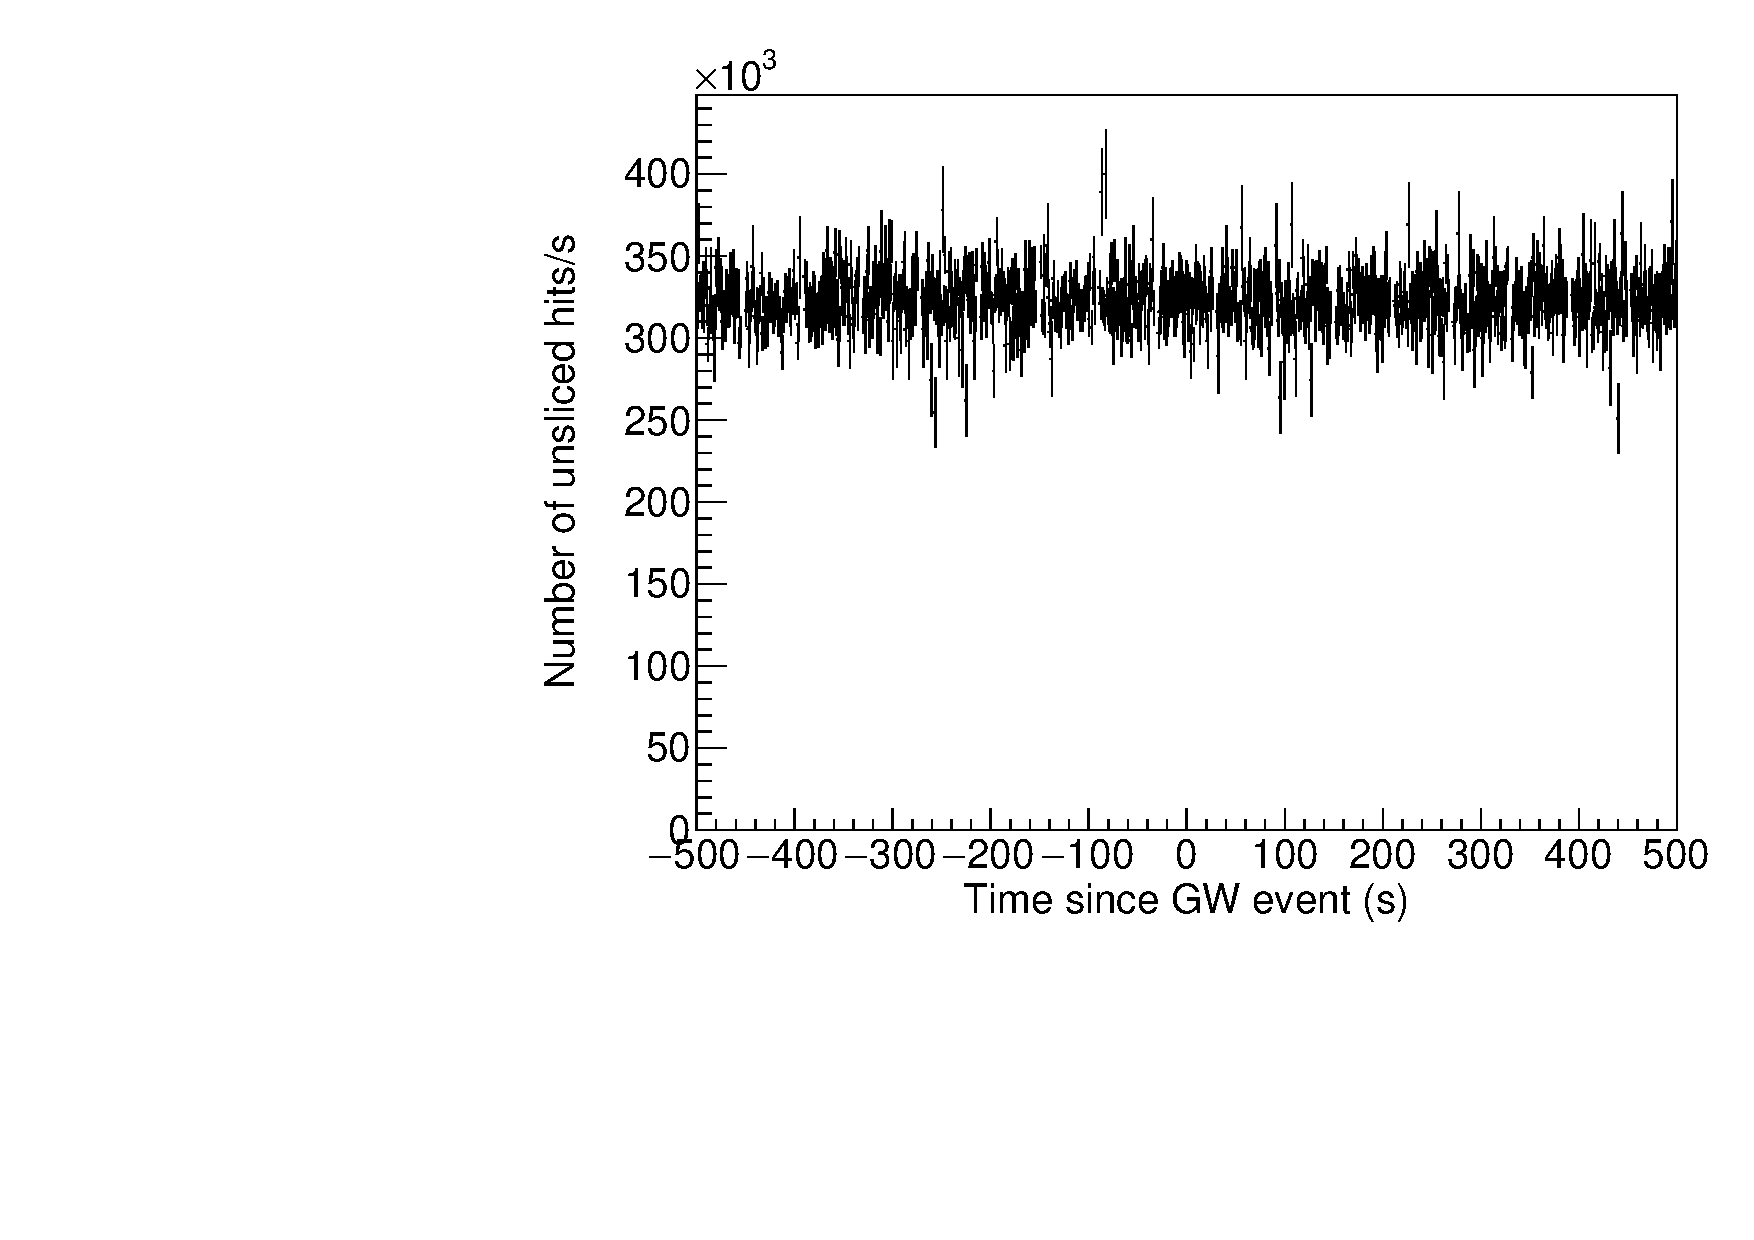
\includegraphics[width=0.333\columnwidth]{ligopass2-neardet-bnb-unslicedhits.pdf}

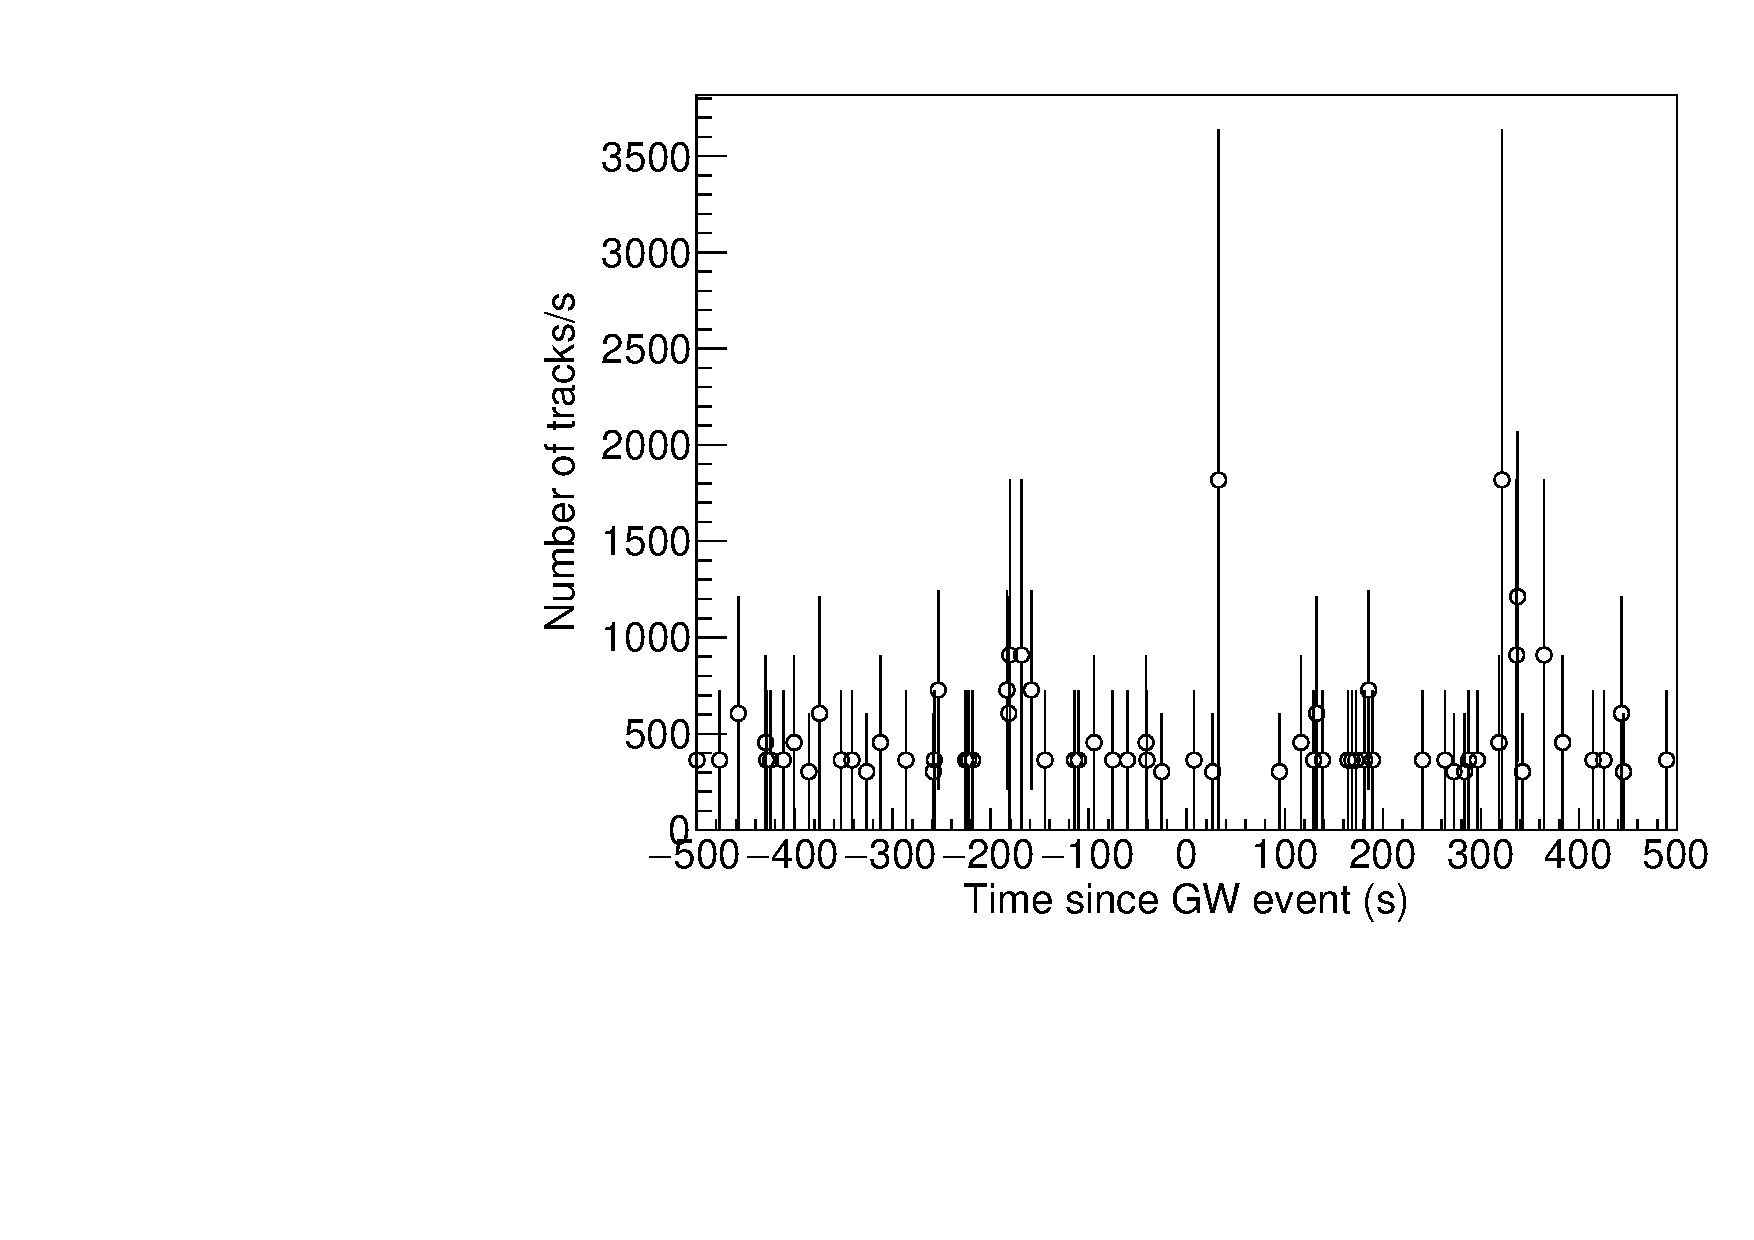
\includegraphics[width=0.333\columnwidth]{ligopass2-neardet-bnb-tracks.pdf}%
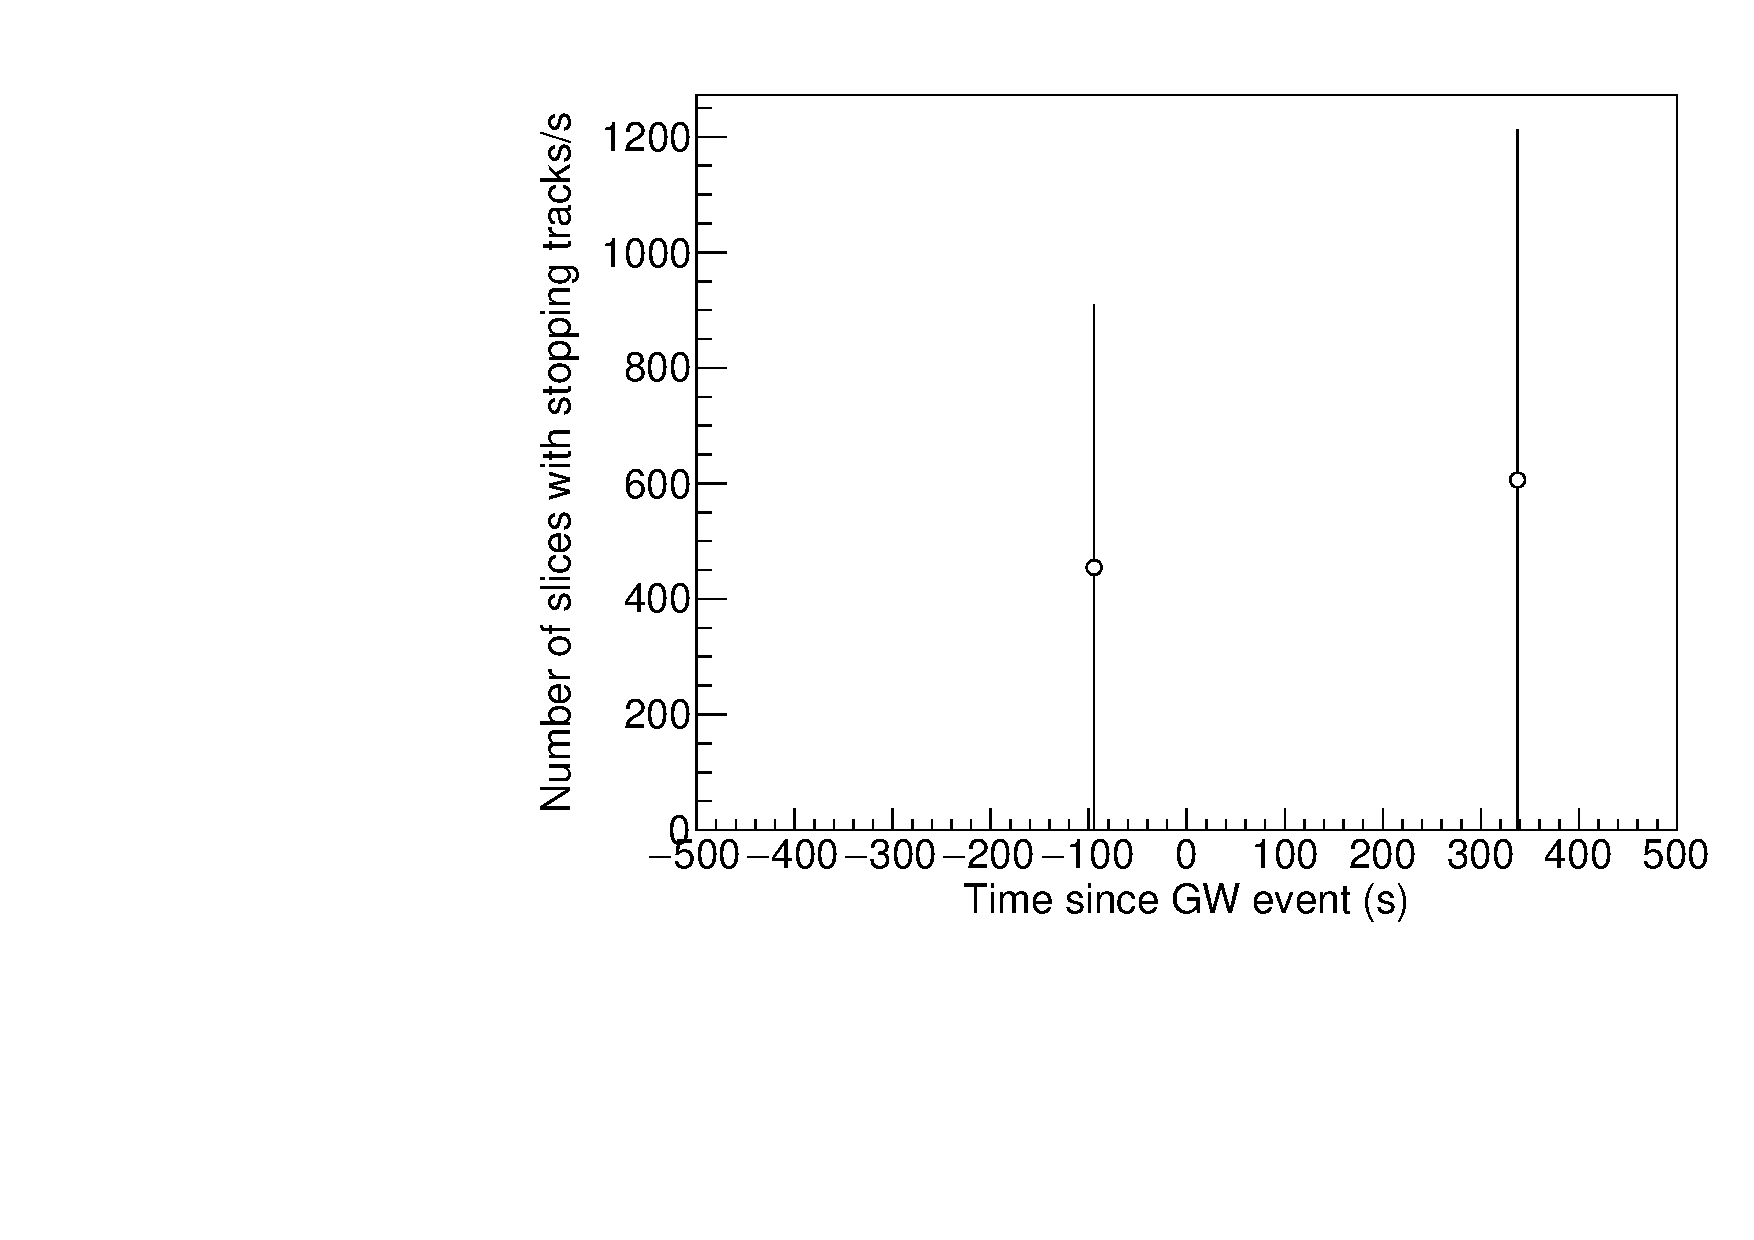
\includegraphics[width=0.333\columnwidth]{ligopass2-neardet-bnb-stoppingtracks.pdf}%
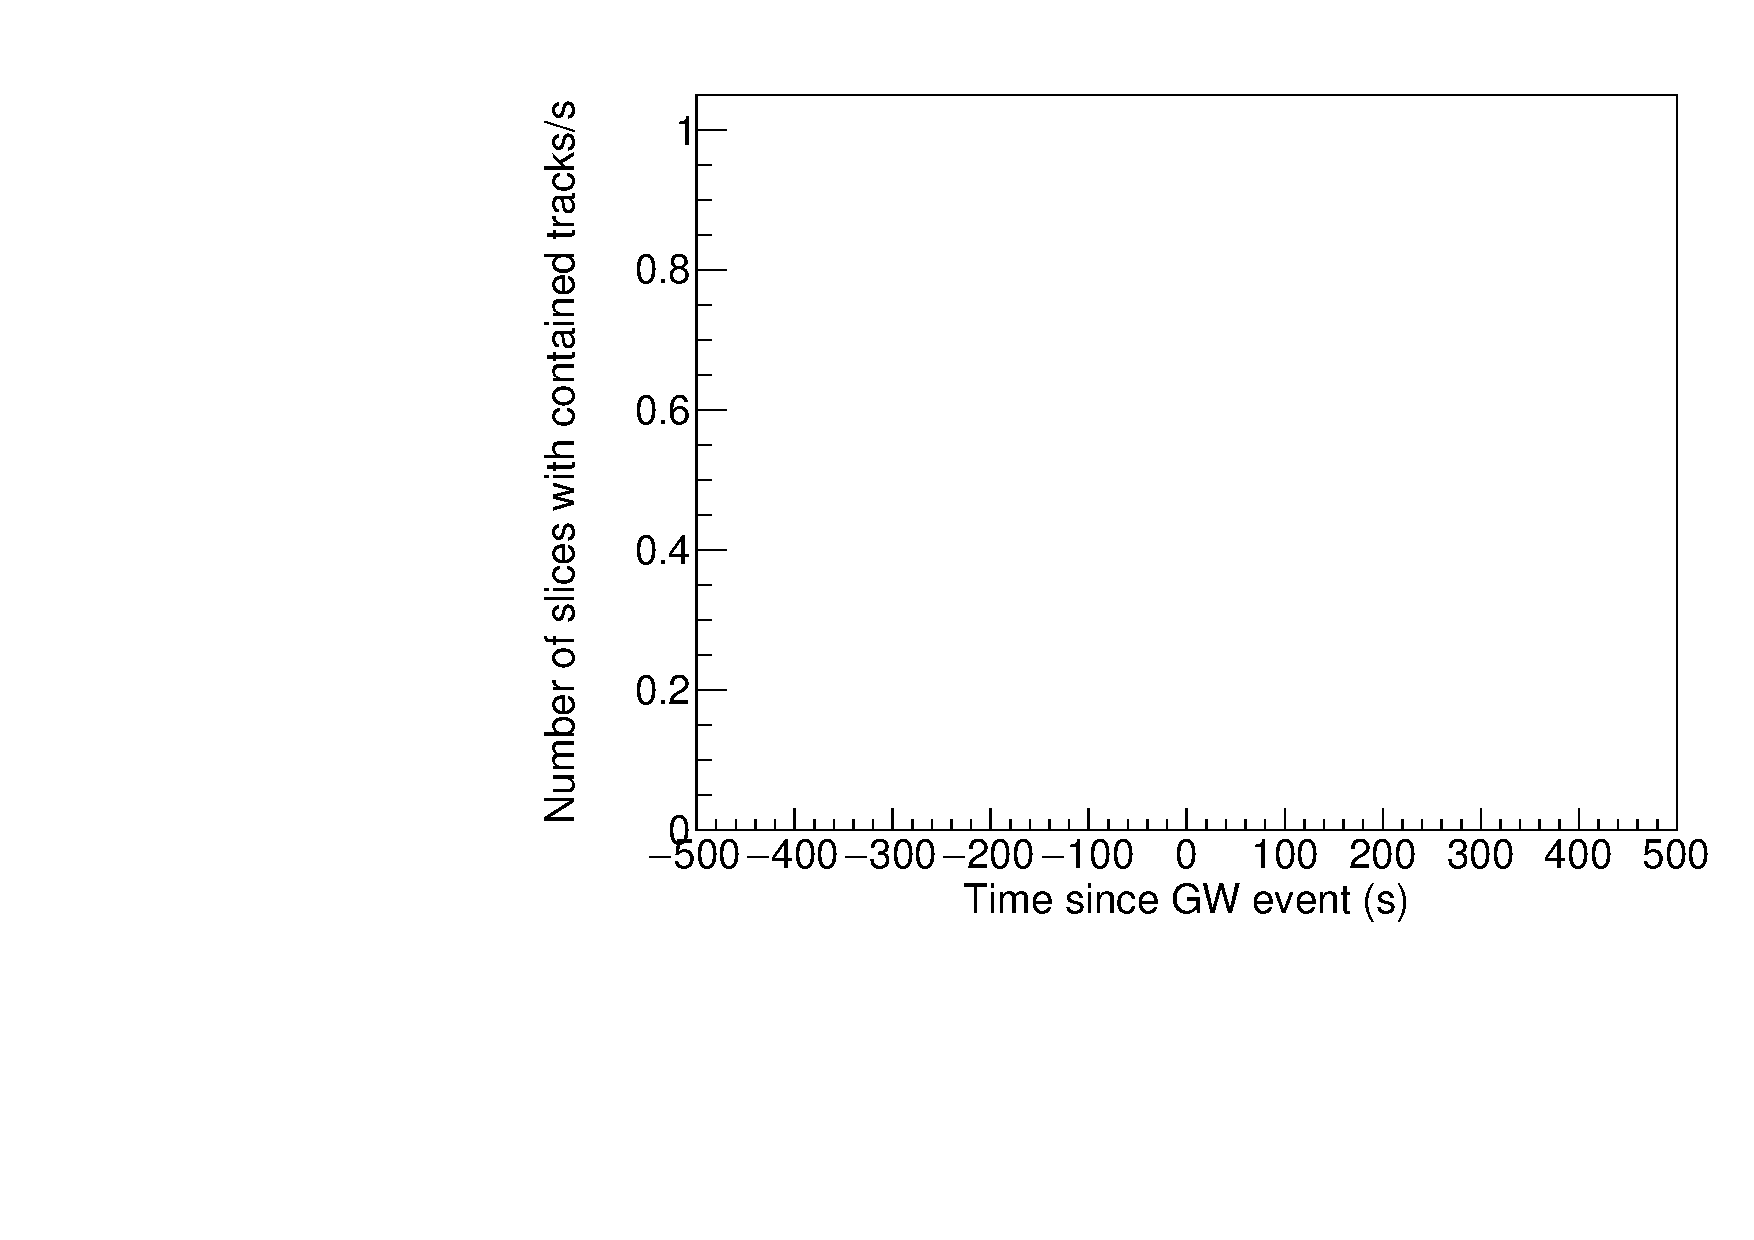
\includegraphics[width=0.333\columnwidth]{ligopass2-neardet-bnb-containedtracks.pdf}%

\end{center}

\ul

  \item BNB livetime isn't very consistent, at least around the test time

\lu

}

\frame{\frametitle{Near Detector ddactivity}

\begin{center}

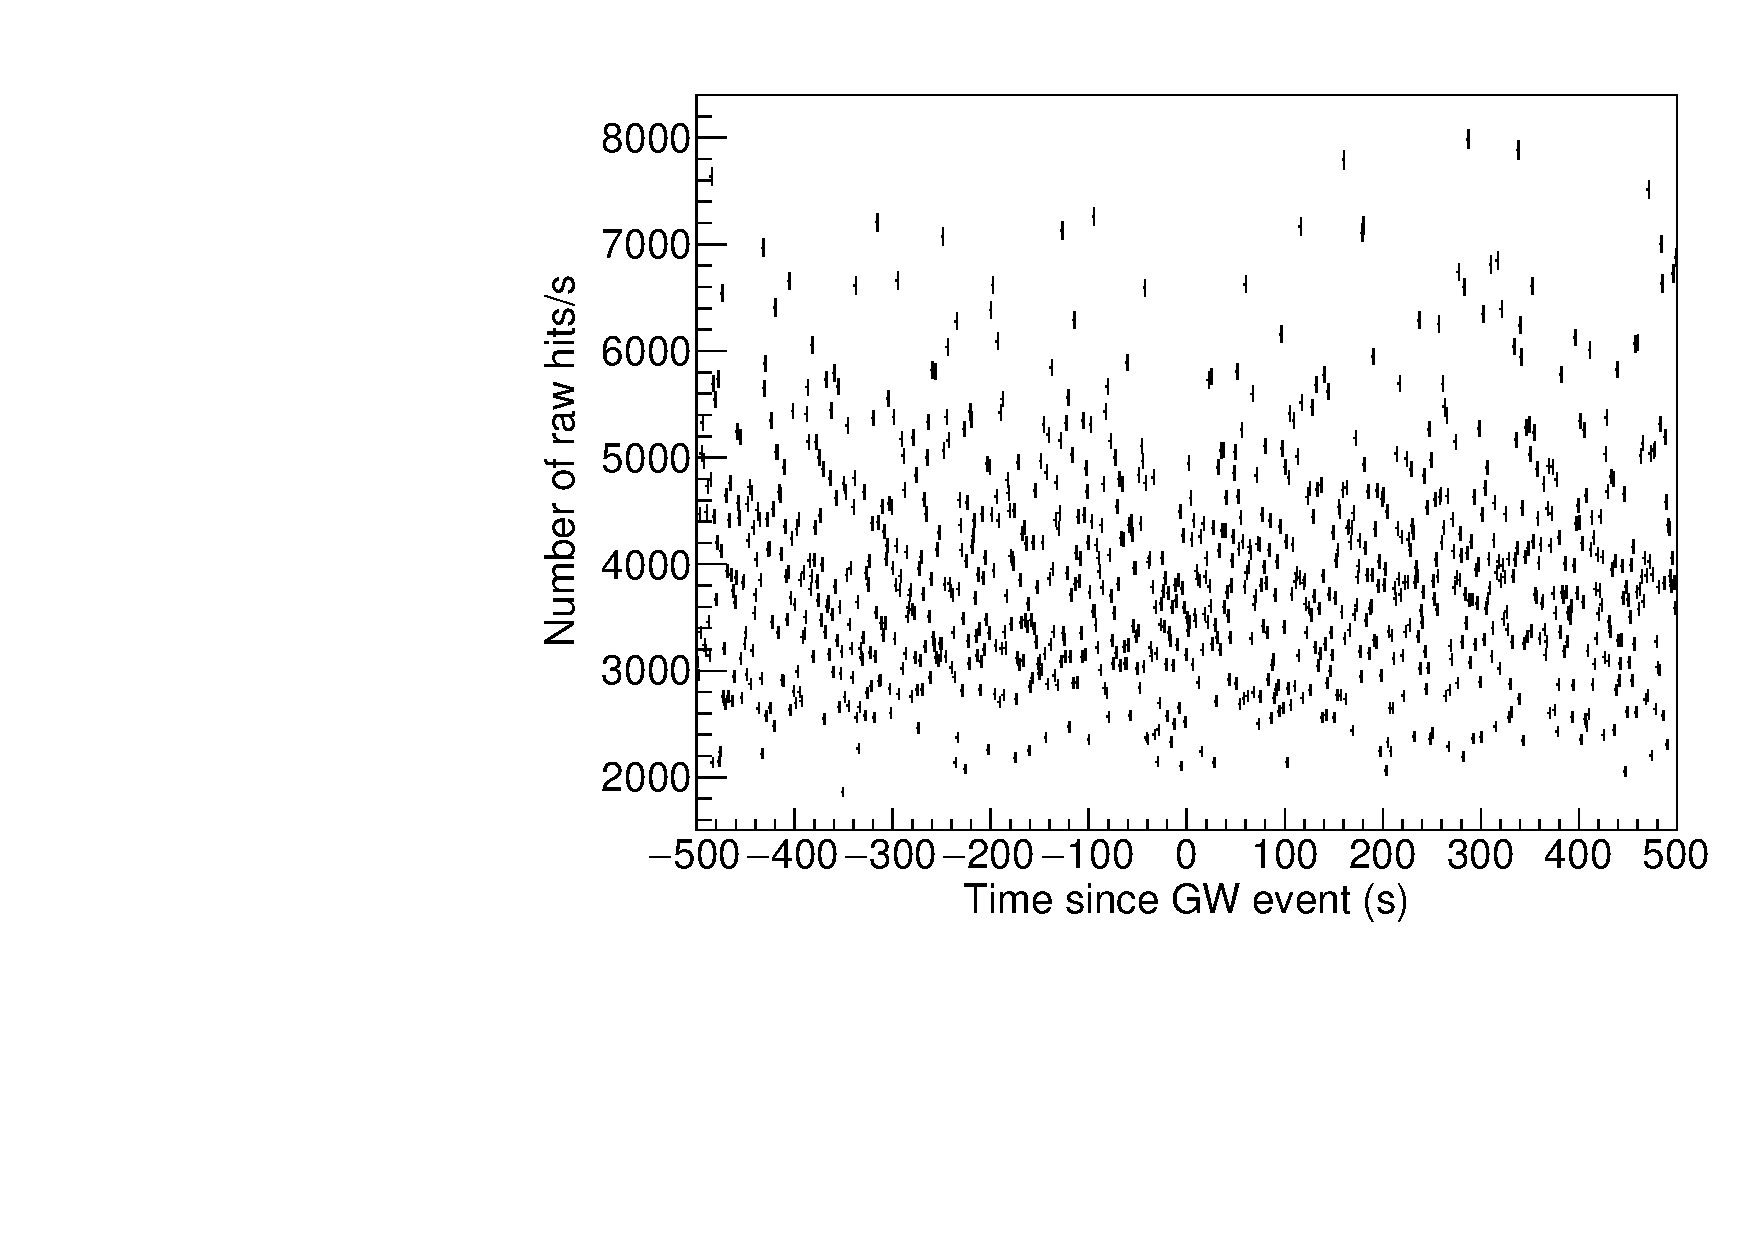
\includegraphics[width=0.333\columnwidth]{ligopass2-neardet-ddactivity1-rawhits.pdf}%
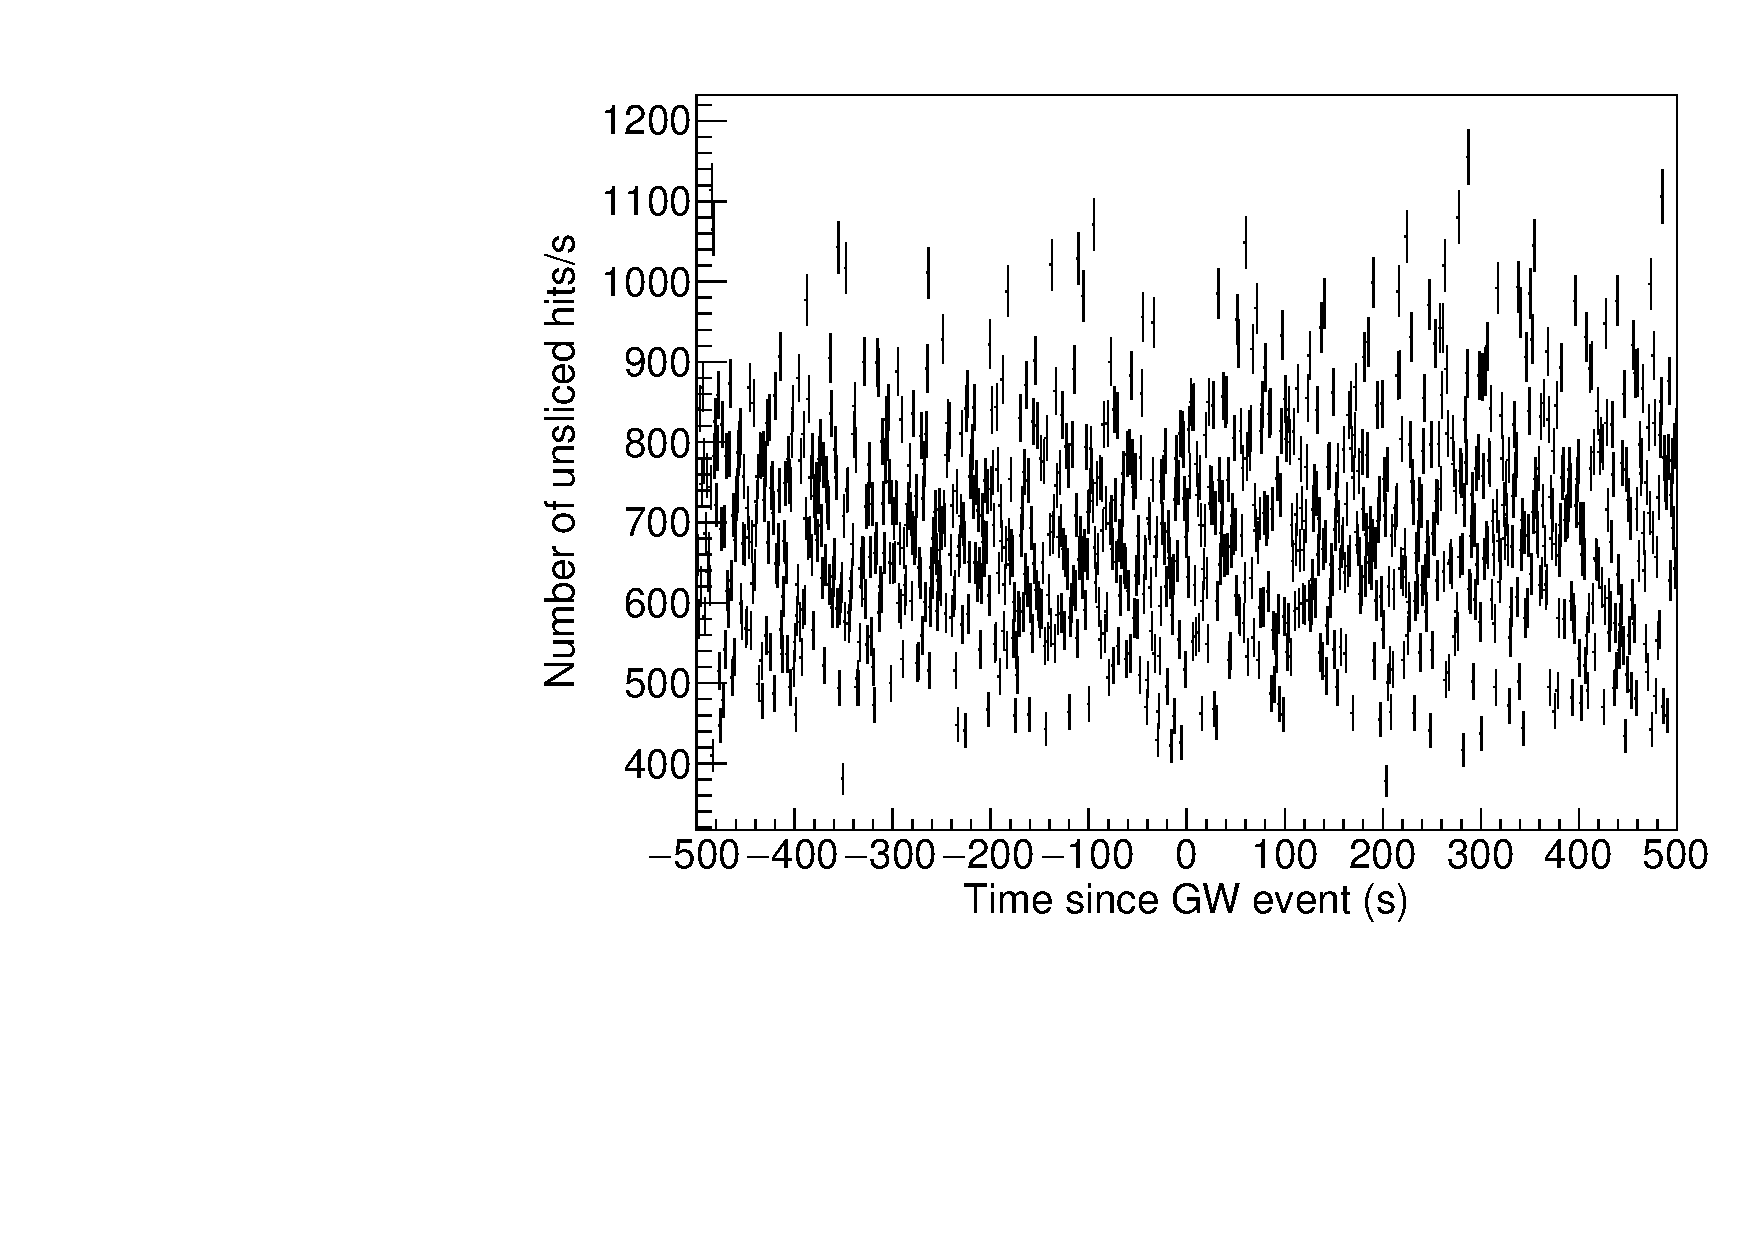
\includegraphics[width=0.333\columnwidth]{ligopass2-neardet-ddactivity1-unslicedhits.pdf}

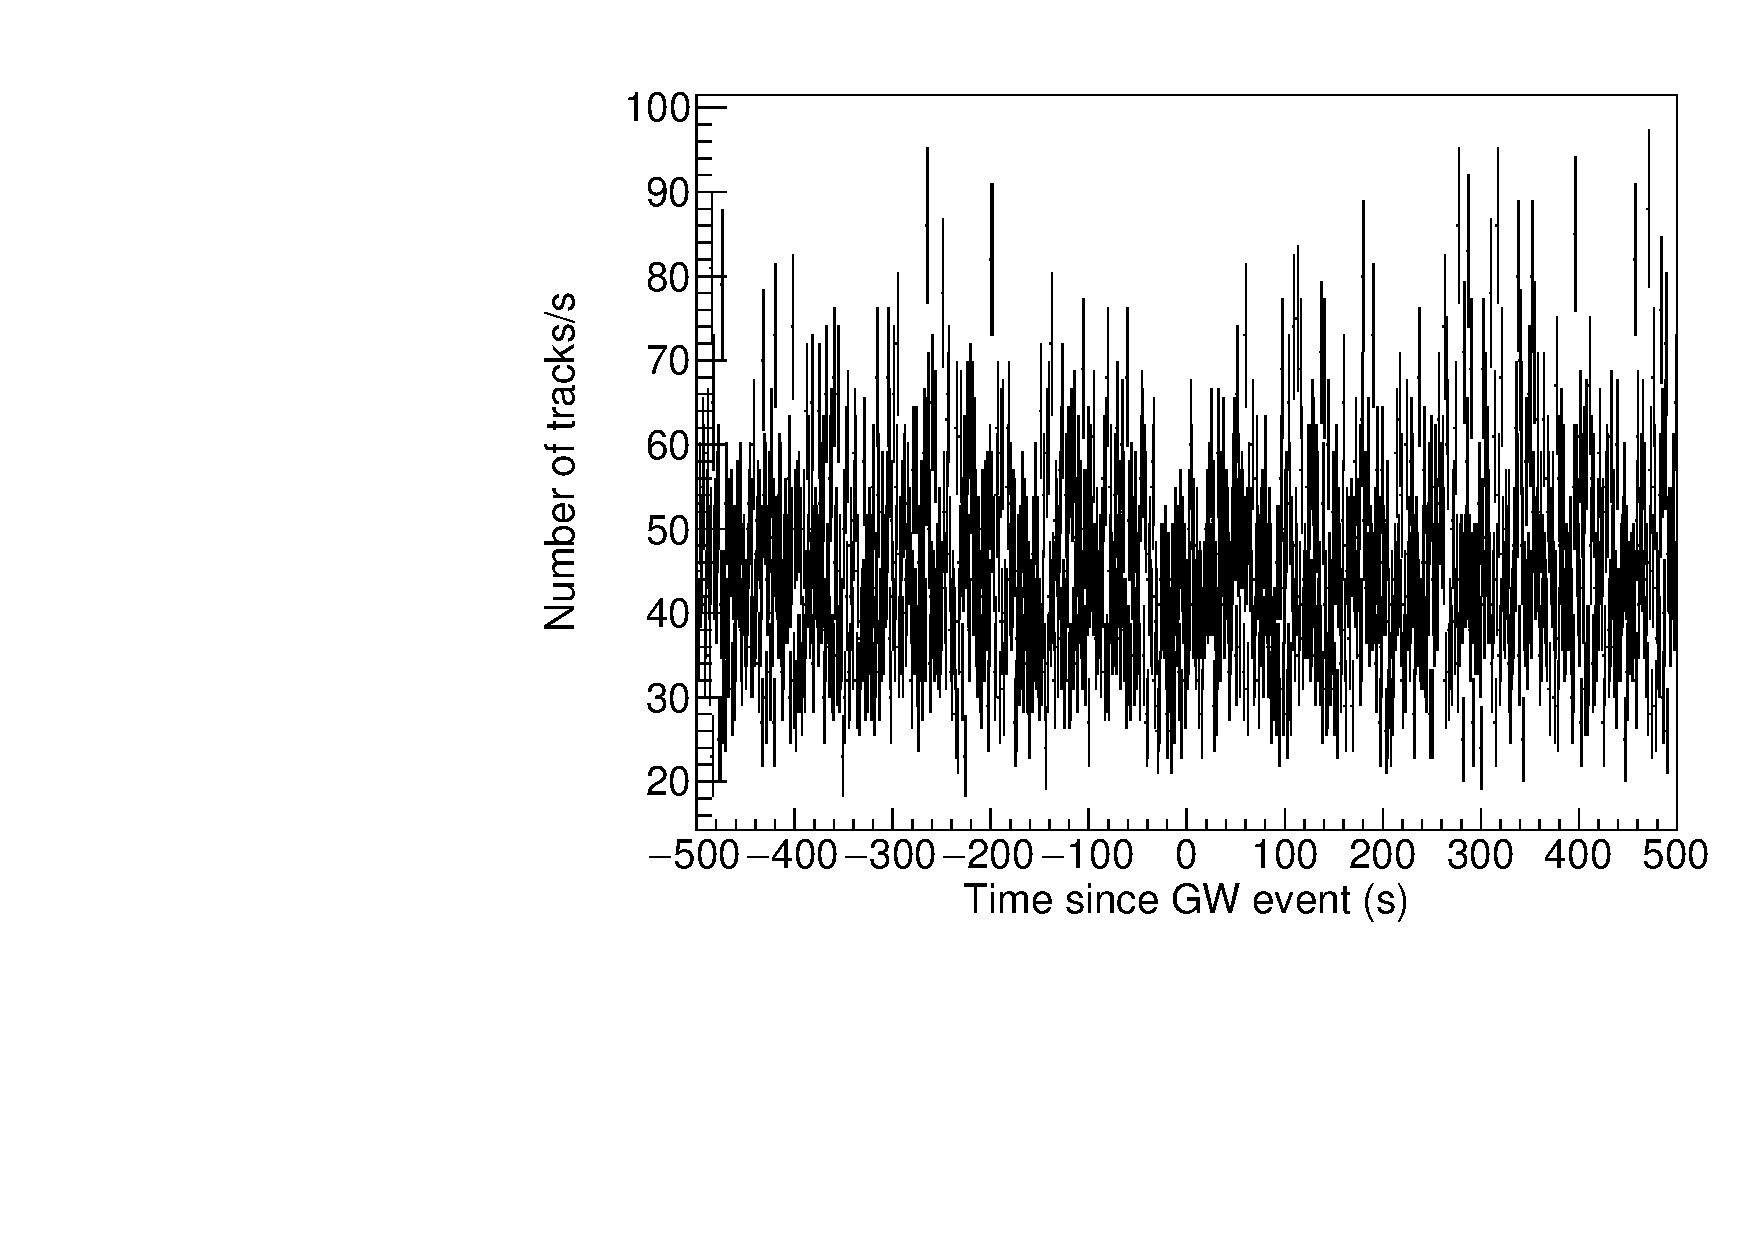
\includegraphics[width=0.333\columnwidth]{ligopass2-neardet-ddactivity1-tracks.pdf}%
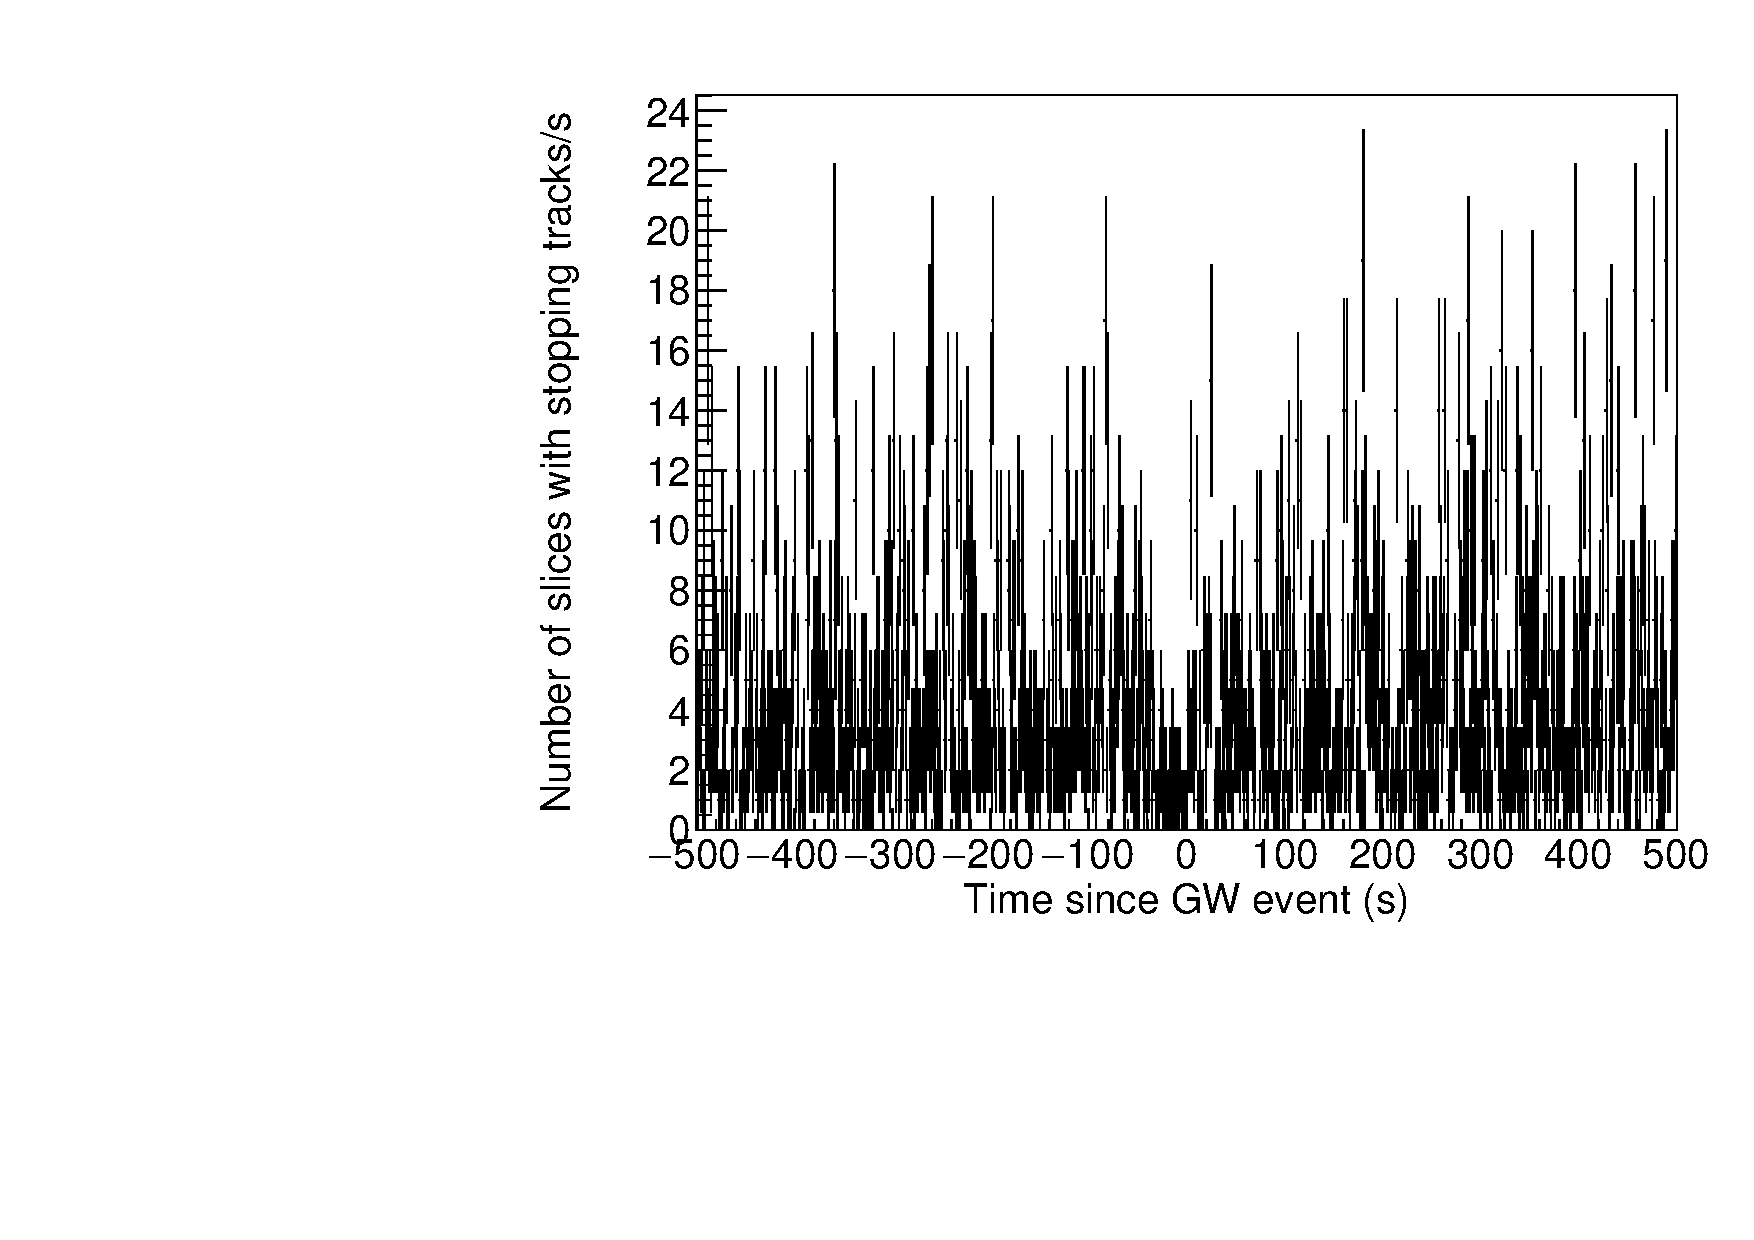
\includegraphics[width=0.333\columnwidth]{ligopass2-neardet-ddactivity1-stoppingtracks.pdf}%
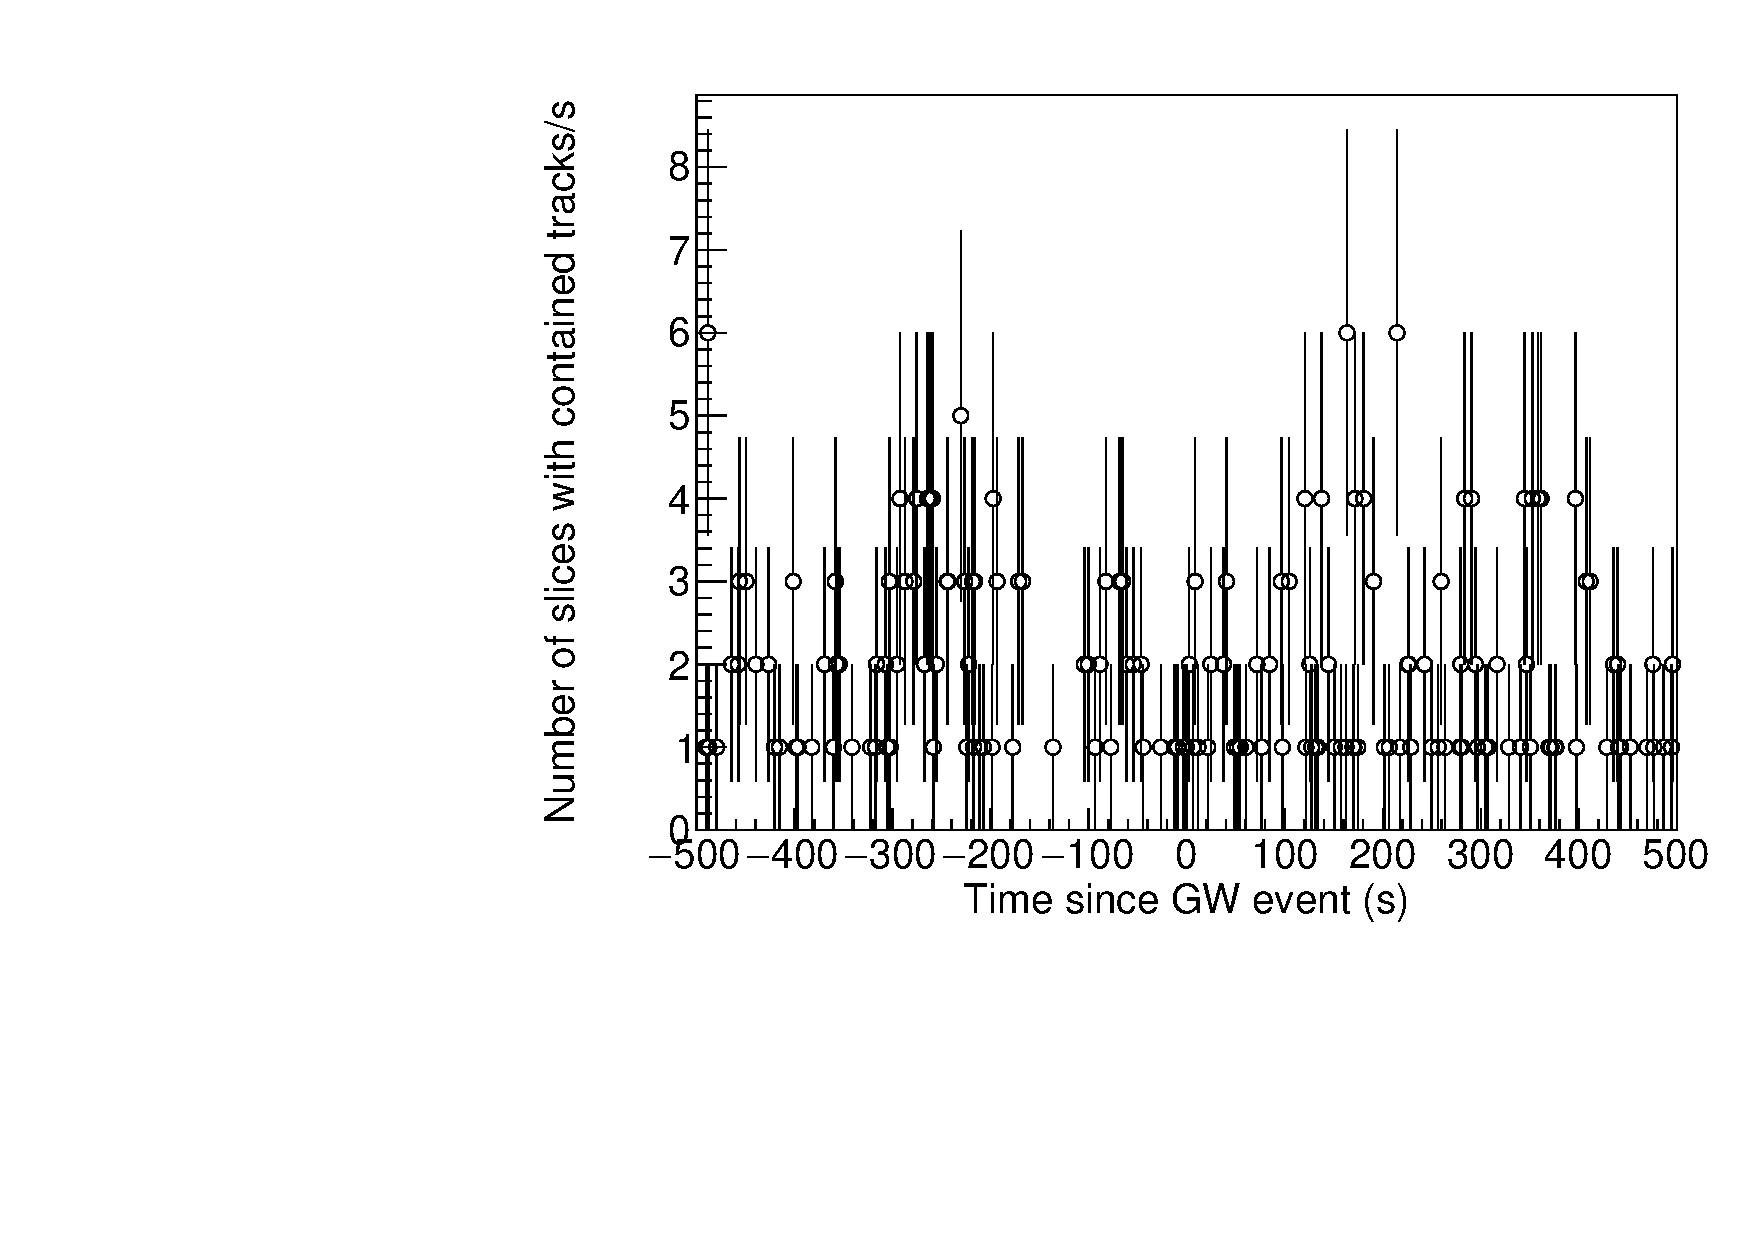
\includegraphics[width=0.333\columnwidth]{ligopass2-neardet-ddactivity1-containedtracks.pdf}%

\end{center}

\ul

  \item \alert{Not} dividing by livetime for this trigger

\lu

}


\section{To do}

\frame{\frametitle{To do}

\ul

\item Flesh out/refine the set of cuts and histograms for each trigger

\ul

  \item Plenty missing currently, e.g. nothing selects contained showers

  \item Want a much better analysis of MeV-scale events.  Will try DDsupernova's 
        slicer

\lu

\item Fit histograms to extract limits

\ul
\item Understand what the acceptance of each trigger is $\Rightarrow$ translate
 raw event count limits to something physical
\lu

\item Repeat test on O(50) randomly chosen times

\item Request box opening

\item Write paper

\lu

}

\beginbackup

\section{Backup}

\frame{\frametitle{Backups}}

\frame{\frametitle{So far}

\ul

\item Alec took a look our data coincident with the first
LIGO event in \href{http://nova-docdb.fnal.gov:8080/cgi-bin/ShowDocument?docid=14351}{doc-14351}

\item Was on 2015-09-14, during shutdown.


  \ul

    \item FD was up, but ``ratty'', in Alec's words.

    \item ND was running smoothly.

  \lu


\item 2nd good LIGO event on 2015-12-26 3:38:53 UTC:

  \ul
  \item Both detectors running smoothly.
  \lu

\item 3rd good LIGO event on 2017-01-04 10:11:58.6 UTC

  \ul
  \item Both detectors running smoothly.
  \lu

\item Marginal LIGO event on 2016-10-12 9:54:43 UTC

  \ul
  \item FD down ``Error in DataLogger''. 
  \item ND ok.
  \lu

\lu

}

\frame{\frametitle{Black hole/black hole mergers}

\begin{center}
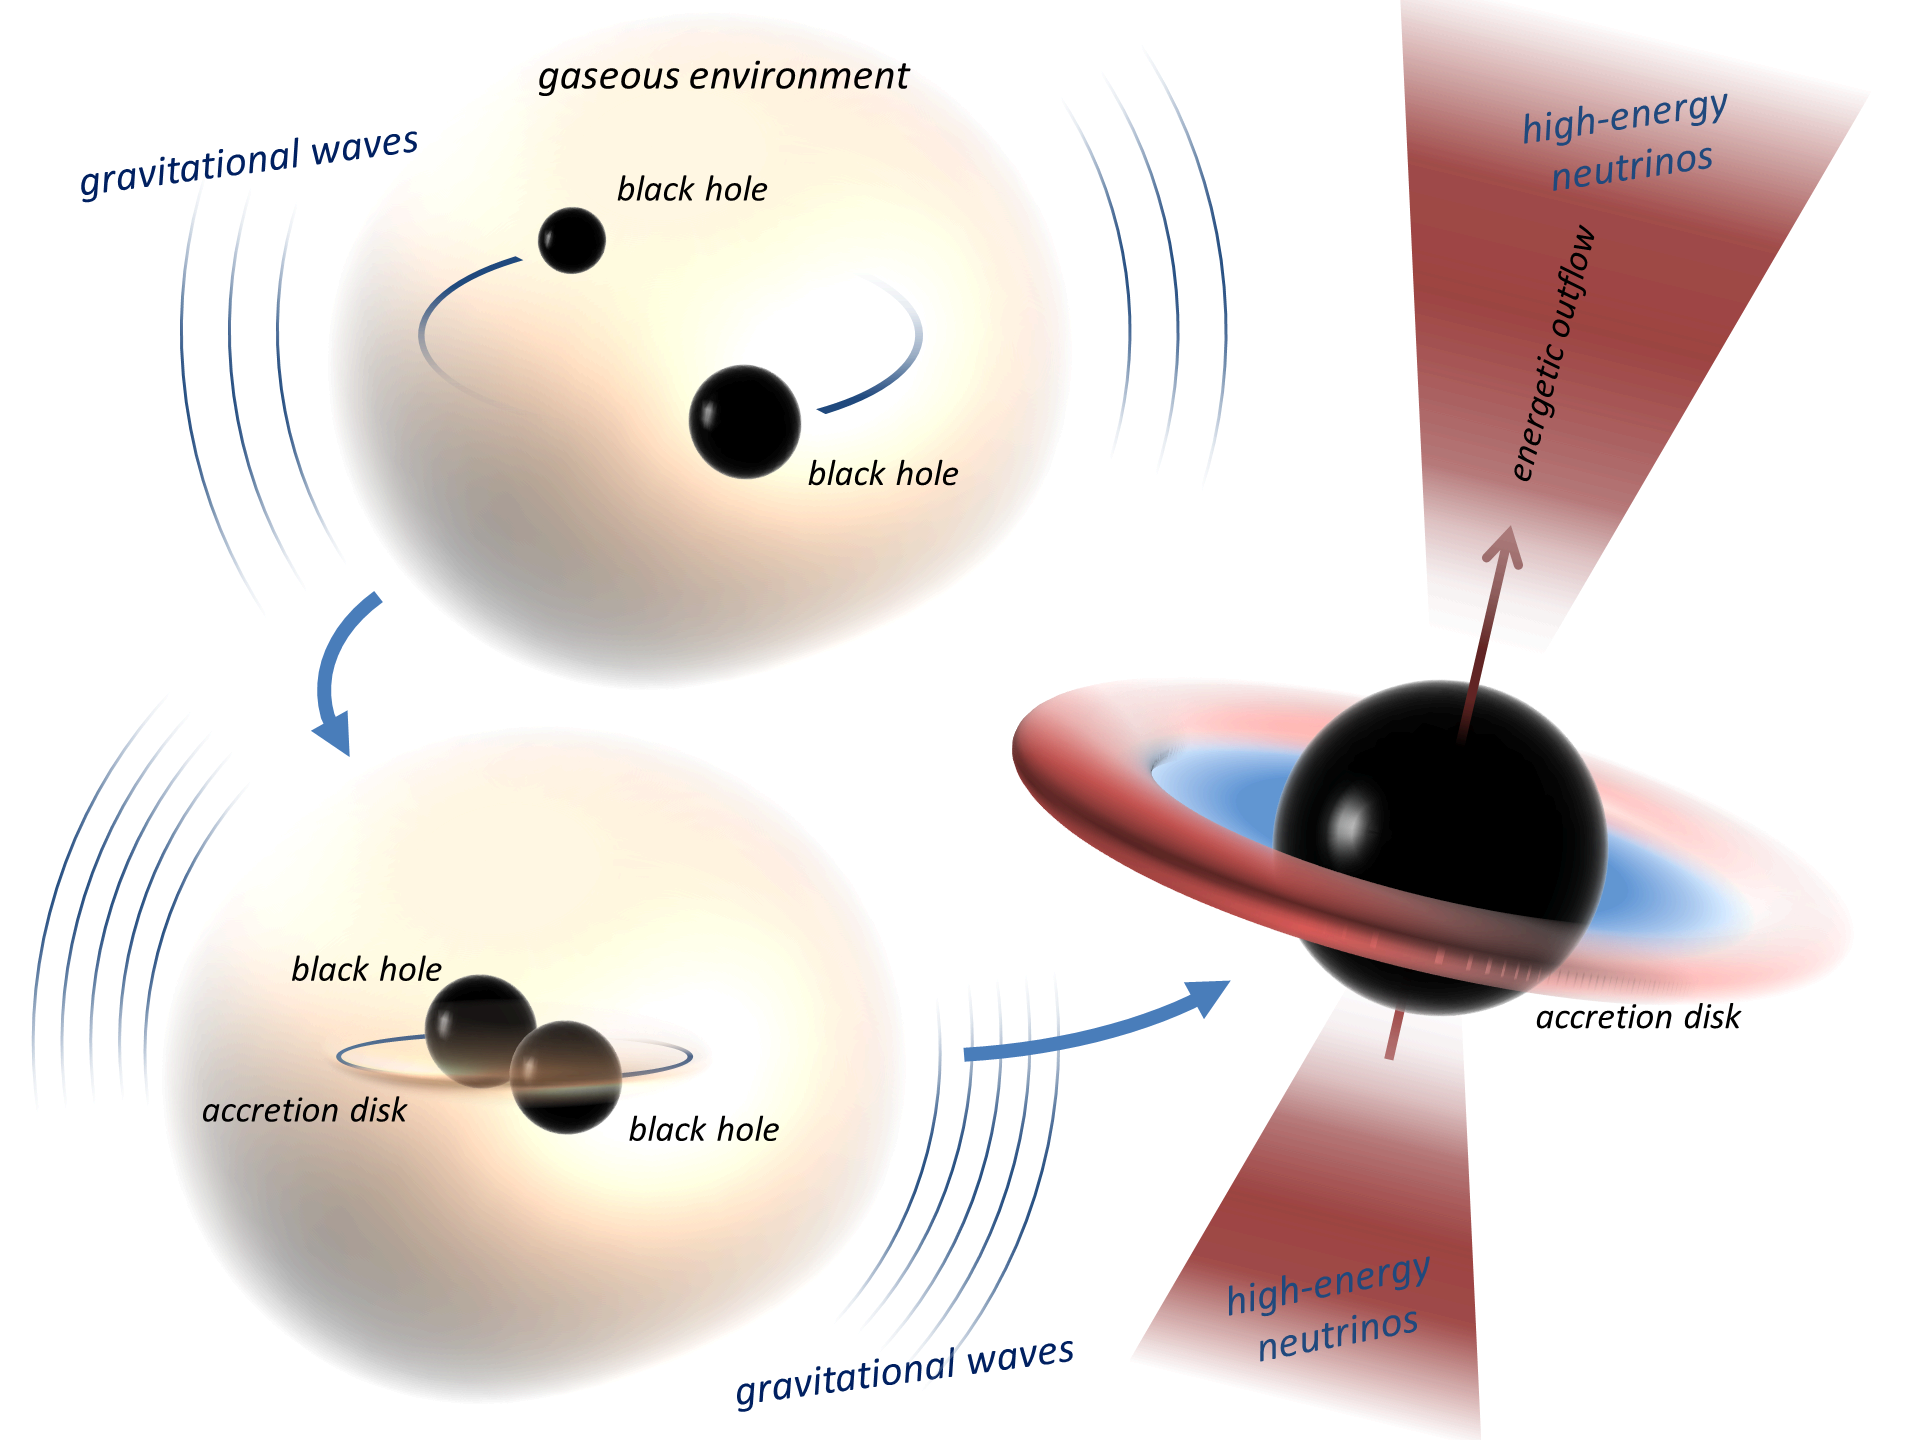
\includegraphics[width=0.5\columnwidth]{fig-bhbh-nu-64.png}
\end{center}

\ul

\item .

\lu

}
\backupend
%%%%%%%%%%%%%%%%%%%%%%%%%%%%%%%%%%%%%%%%%%%%%%%%%%%%%%%%%%%%%%%%%%%%%%%%
\end{document}
